\documentclass[12pt,t]{beamer}

\setbeamersize{text margin left=0pt, text margin right=4cm}
\hypersetup{colorlinks=true,linkcolor=red}
\usetheme{boxes}

\usepackage[utf8]{inputenc}
\usepackage[russian,english]{babel}
\usepackage[T2A]{fontenc}
\usepackage{hyperref}
\usepackage[final]{listings}
\usepackage{breakurl}
\usepackage{cite}
\usepackage{perpage}

\graphicspath{{img/}}

\def\Url\Breaks{\do\/\do-}
\lstset{
  frame=single,
  breaklines=true,
  basicstyle=\small,
  postbreak=\raisebox{0ex}{\ensuremath{\hookrightarrow\space}},
  numbers=left
}

\MakePerPage{footnote}

\title{Операционные Системы}
\subtitle{Алгоритмы аллокации памяти}
\date{\today}

\begin{document}

  \begin{frame}
    \titlepage
  \end{frame}
  \begin{frame}[fragile]
\frametitle{Аллокация памяти}
\begin{itemize}
    \item<1->Рассмотрим простейшую постановку задачи:
    \begin{itemize}
        \item<2->есть непрерывный участок логической памяти;
        \item<3->функция аллокации: \lstinline|void *alloc(int size)|;
        \item<4->функция освобождения: \lstinline|void free(void *free)|.
    \end{itemize}
\end{itemize}
\end{frame}

\begin{frame}
\frametitle{Выравнивание}
\begin{itemize}
    \item<1->Некоторые процессоры требуют выравненных указателей
    \begin{itemize}
        \item<2->2 байта - выравнивание 2 байта;
        \item<3->4 байта - выравнивание 4 байта;
        \item<4->8 байт - выравнивание 8 байт...
    \end{itemize}
\end{itemize}
\end{frame}

\begin{frame}
\frametitle{Простой подход к аллокации}
\begin{itemize}
    \item<1->Создадим связный список свободных блоков
    \begin{itemize}
        \item<1->каждый узел списка описывает непрерывный свободный участок;
        \item<2->узлы списка хранятся в начале каждого свободного блока.
    \end{itemize}
\end{itemize}
\end{frame}

\begin{frame}
\frametitle{Связный список свободных блоков}
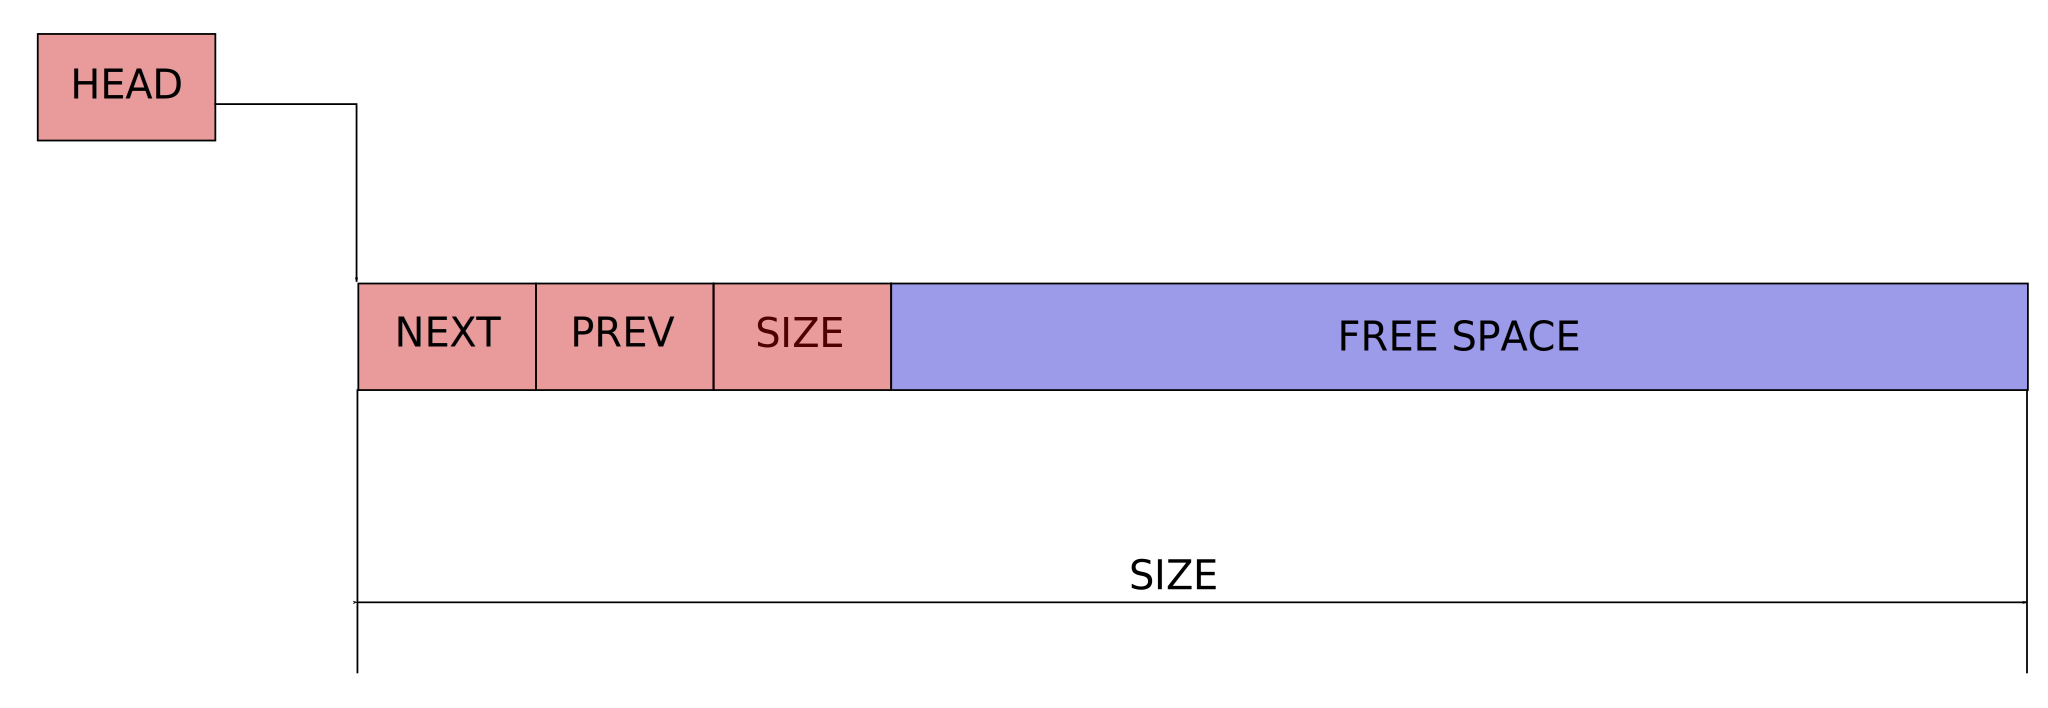
\includegraphics[height=.3\textheight]{lst0}
\end{frame}

\begin{frame}
\frametitle{Аллокация свободного блока}
\begin{itemize}
    \item<1->Пройдемся по списку и найдем блок достаточного размера
    \begin{itemize}
        \item<2->если блок слишком большой, то отрезаем от него часть;
        \item<3->если походящего блока не нашлось, то возвращаем ошибку.
    \end{itemize}
\end{itemize}
\end{frame}

\begin{frame}
\frametitle{Аллокация свободного блока}
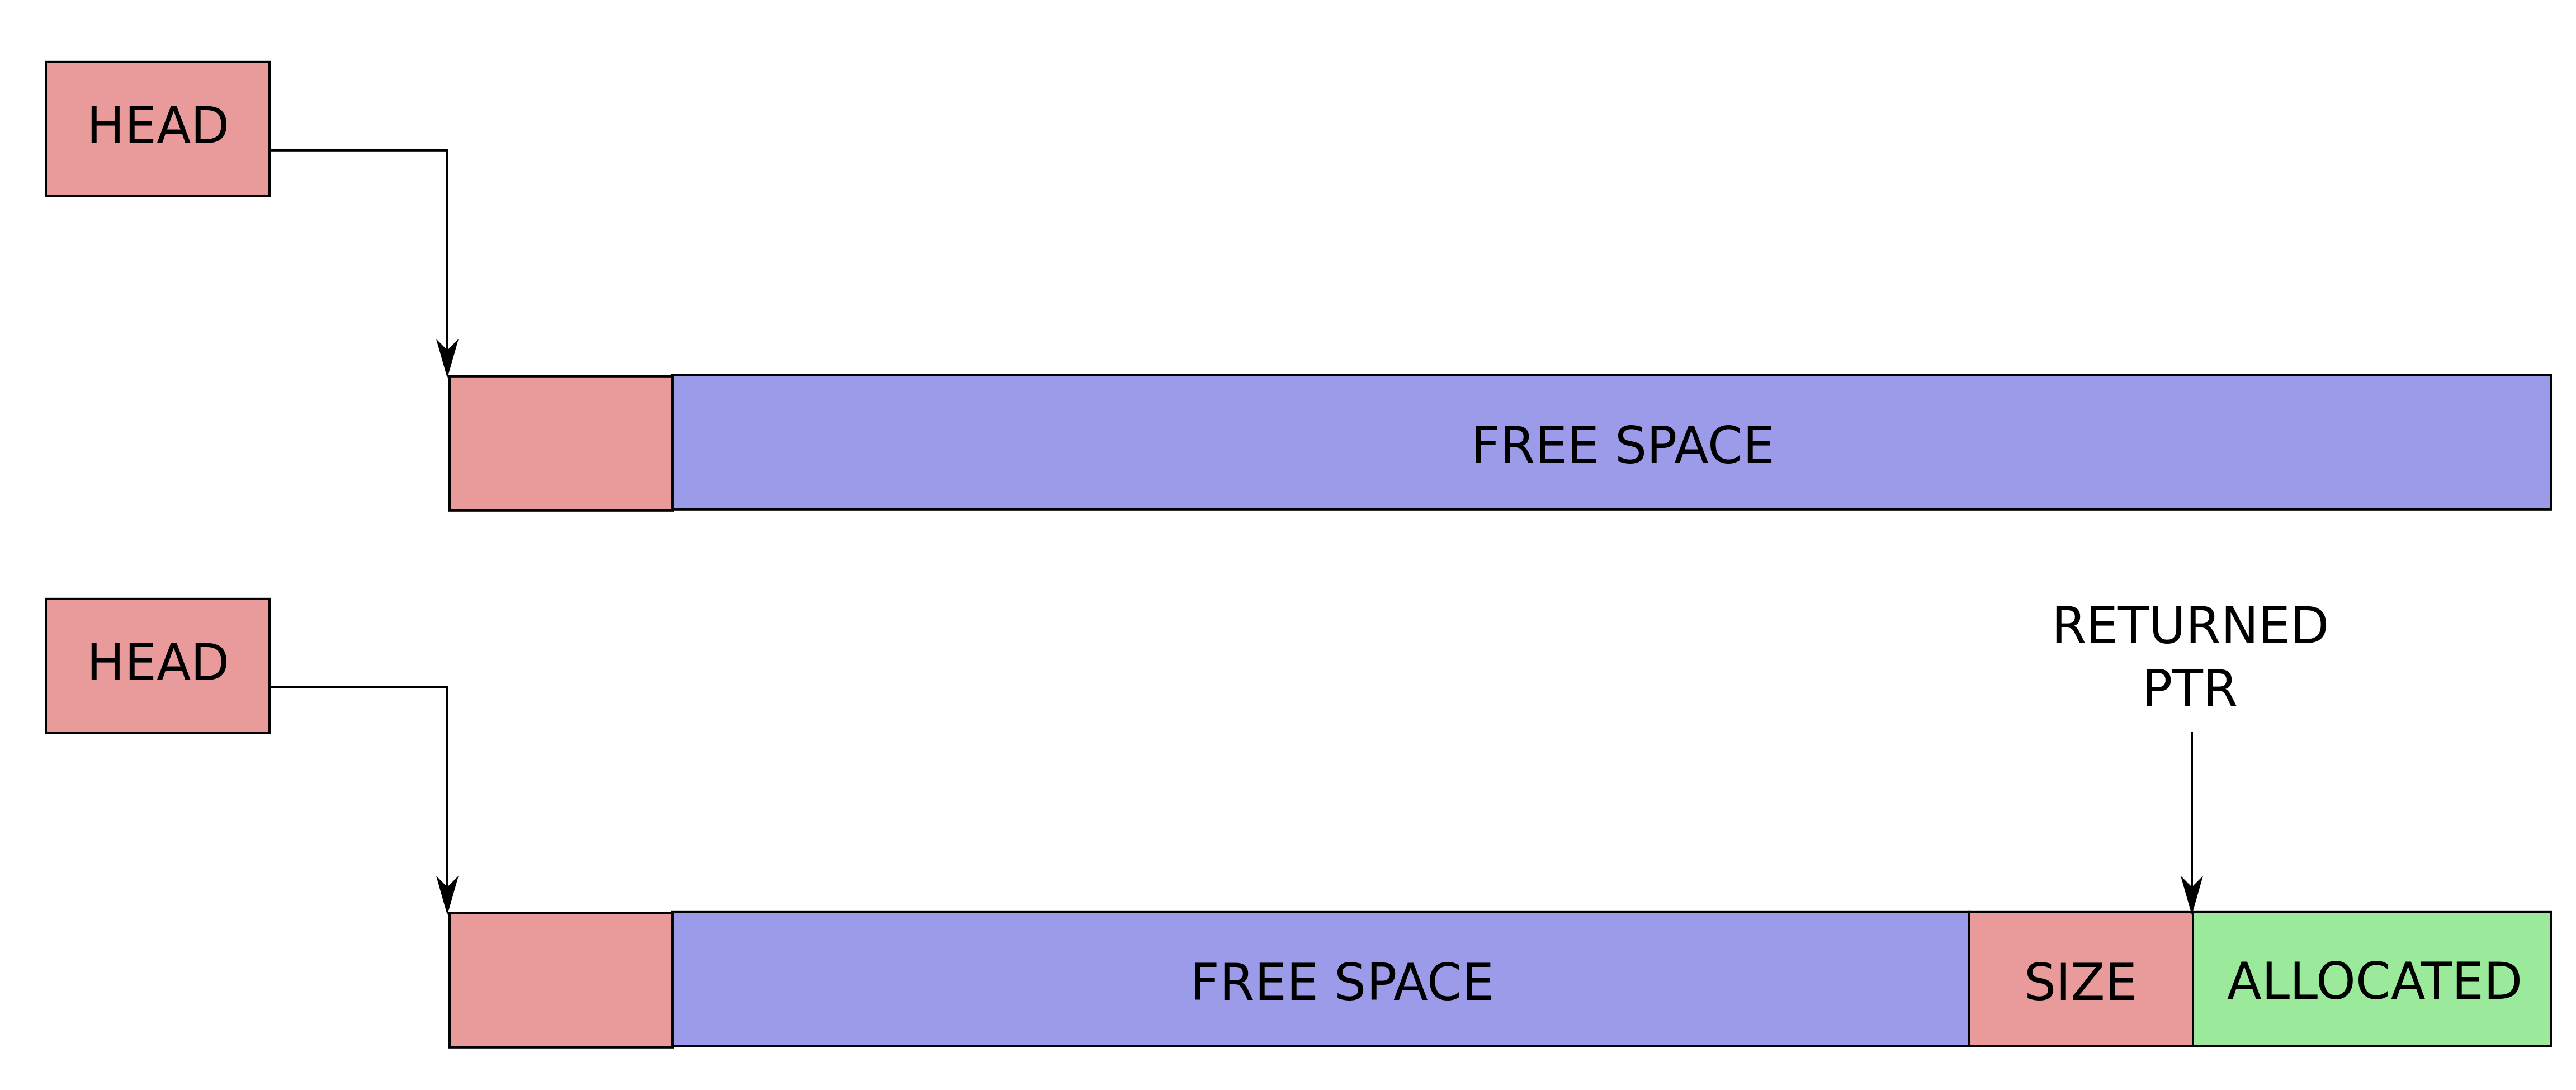
\includegraphics[height=.4\textheight]{lst1}
\end{frame}

\begin{frame}
\frametitle{Освобождение занятого блока}
\begin{itemize}
    \item<1->Чтобы освободить свободный блок, его нужно вернуть в список
    \begin{itemize}
        \item<2->например, можно добавить в список новый элемент.
    \end{itemize}
\end{itemize}
\end{frame}

\begin{frame}
\frametitle{Освобождение занятого блока}
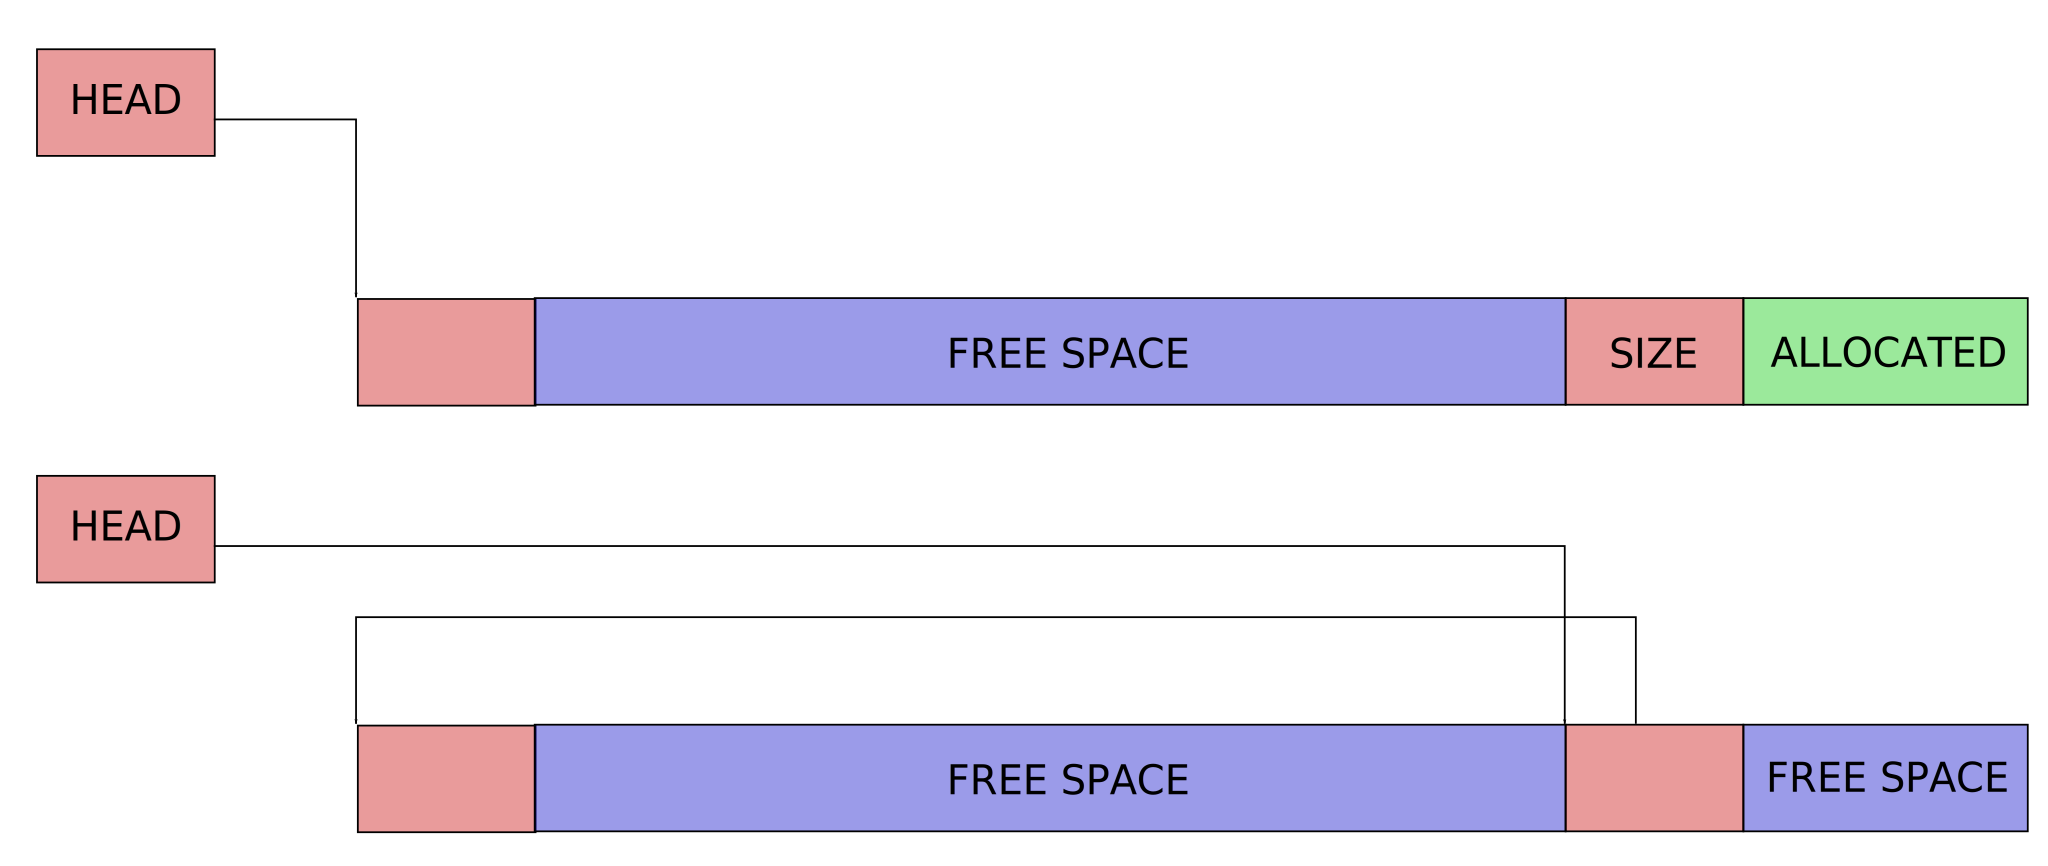
\includegraphics[height=.4\textheight]{lst2}
\end{frame}

\begin{frame}
\frametitle{Фрагментация свободной памяти}
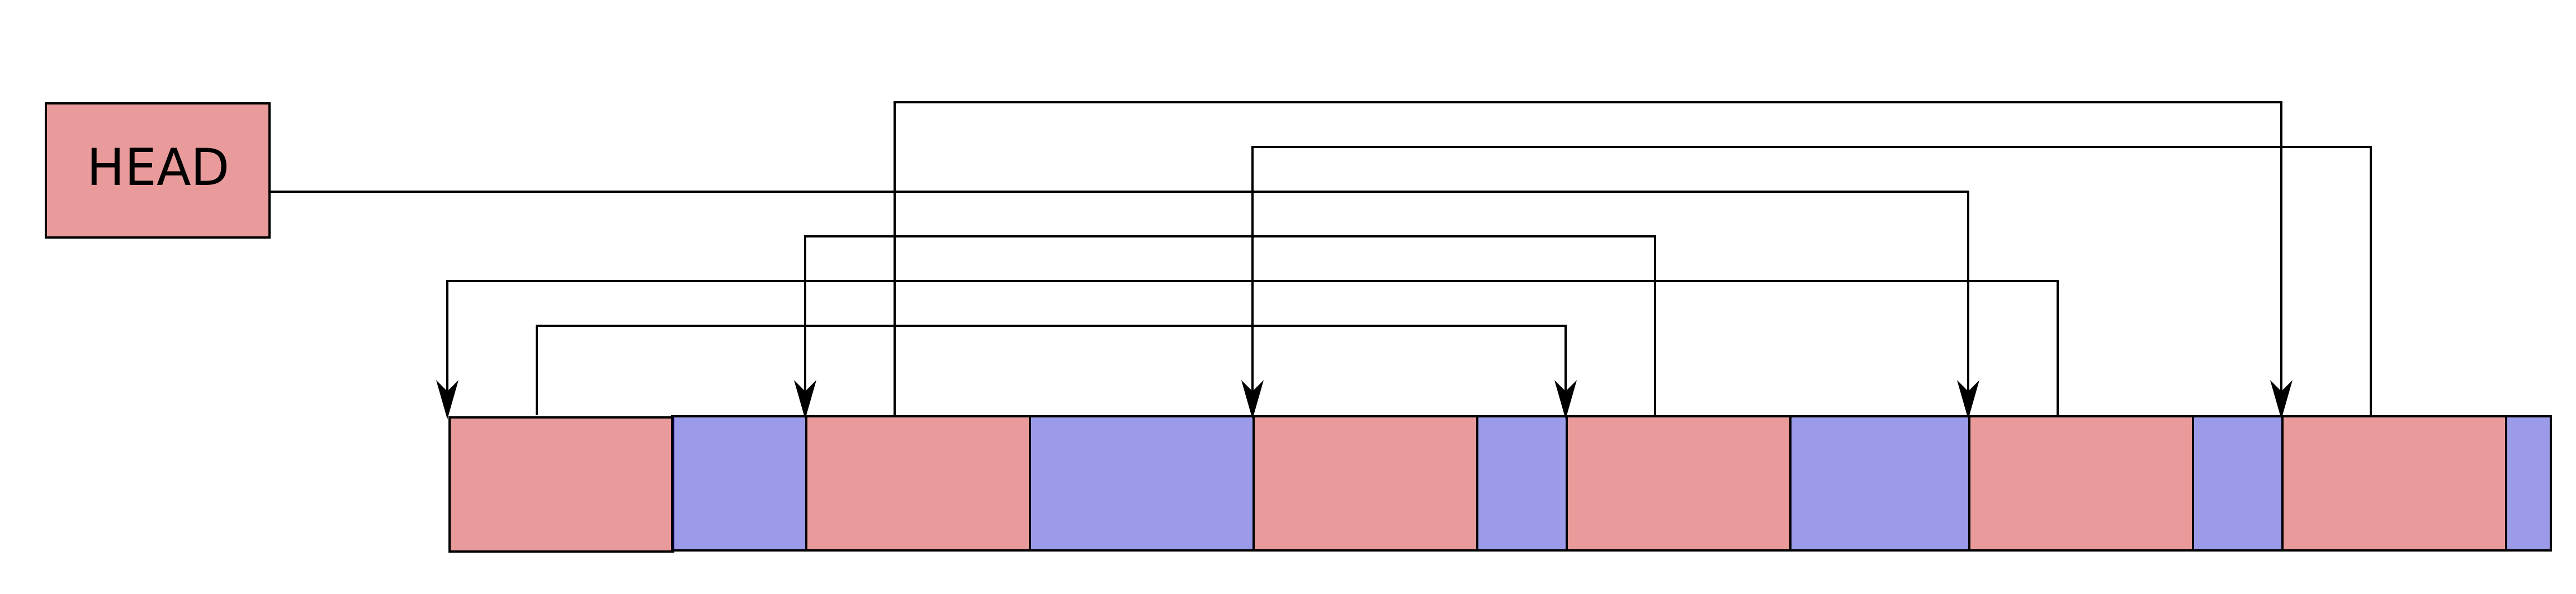
\includegraphics[height=.2\textheight]{lst3}
\end{frame}

\begin{frame}
\frametitle{Боремся с фрагментацией}
\begin{itemize}
    \item<1->Как избежать подобной фрагментации?
    \begin{itemize}
        \item<2->искать смежные блоки проходом по списку ($O\left(N\right)$);
        \item<3->поддерживать список упорядоченным ($O\left(N\right)$);
        \item<4->использовать упорядоченную структуру вместо списка
        ($O\left(log N\right)$);
        \item<5->использовать граничные маркеры (Border Tags,
        $O\left(1\right)$).
    \end{itemize}
\end{itemize}
\end{frame}

\begin{frame}
\frametitle{Граничные маркеры}
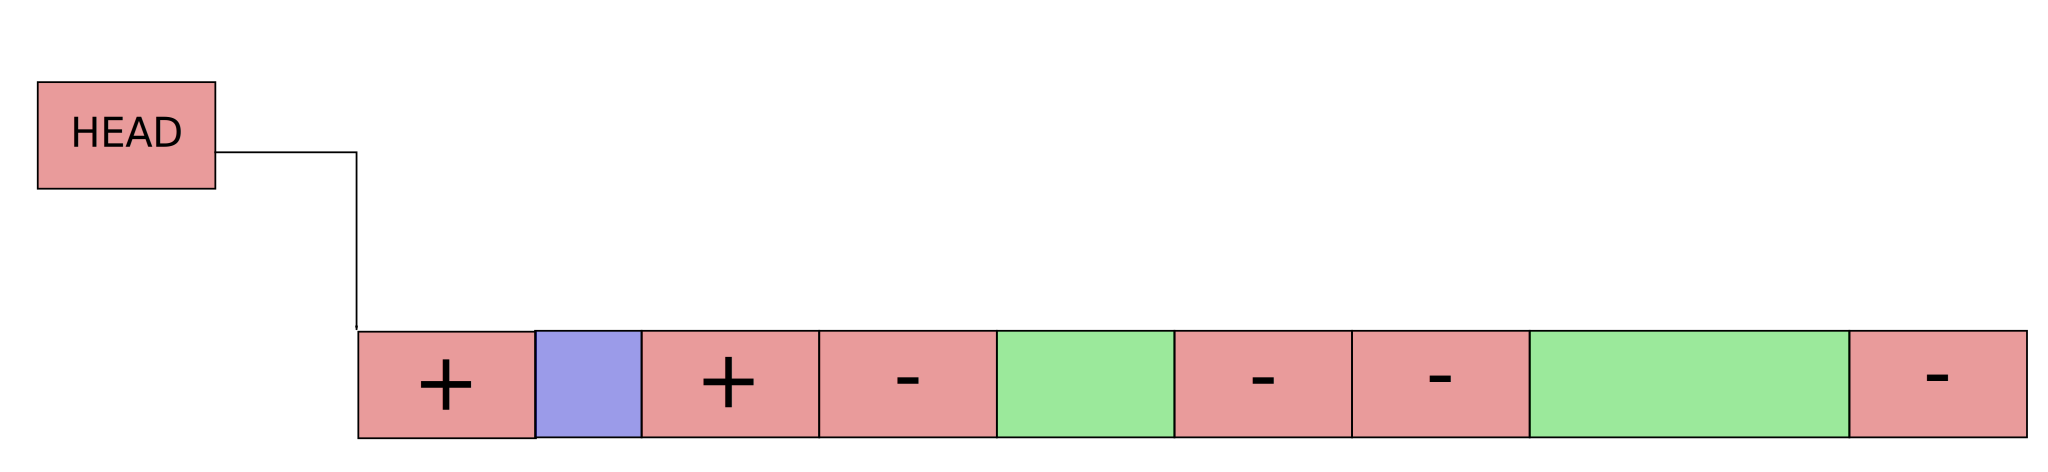
\includegraphics[height=.2\textheight]{lst4}
\end{frame}

\begin{frame}
\frametitle{Граничные маркеры}
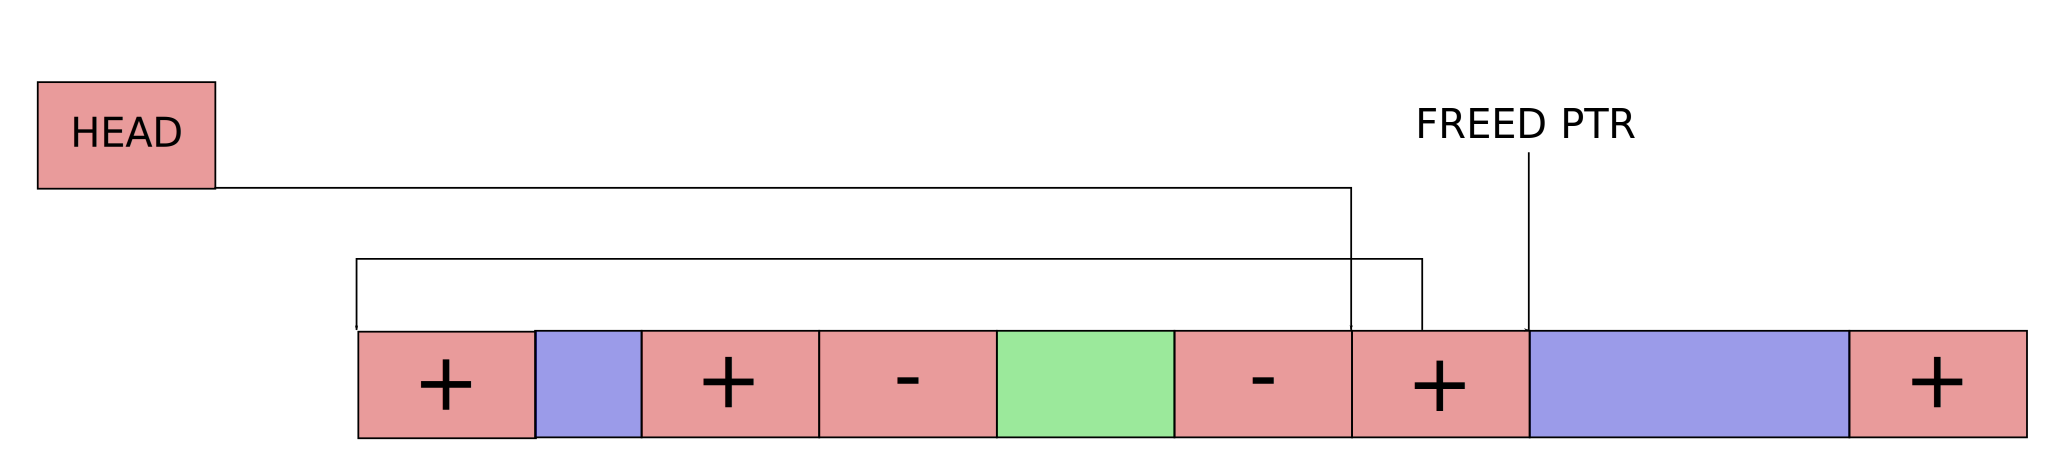
\includegraphics[height=.2\textheight]{lst5}
\end{frame}

\begin{frame}
\frametitle{Граничные маркеры}
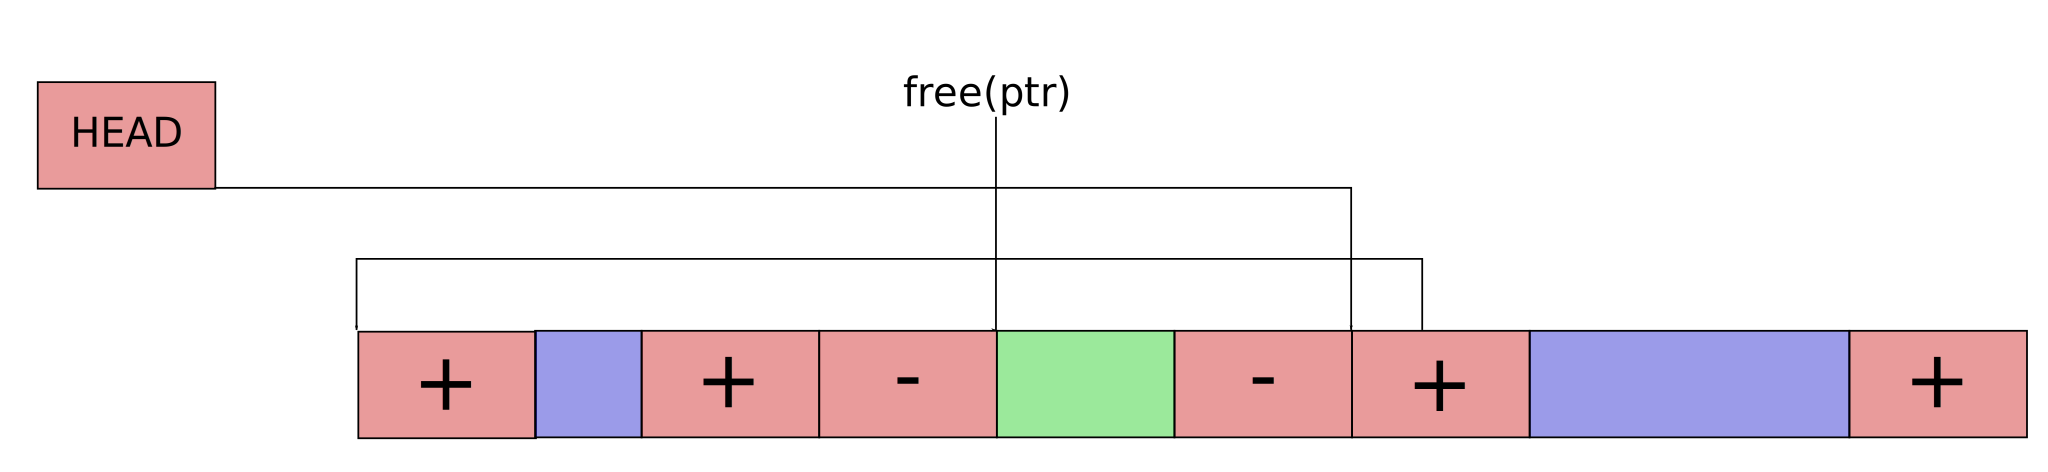
\includegraphics[height=.2\textheight]{lst6}
\end{frame}

\begin{frame}
\frametitle{Граничные маркеры}
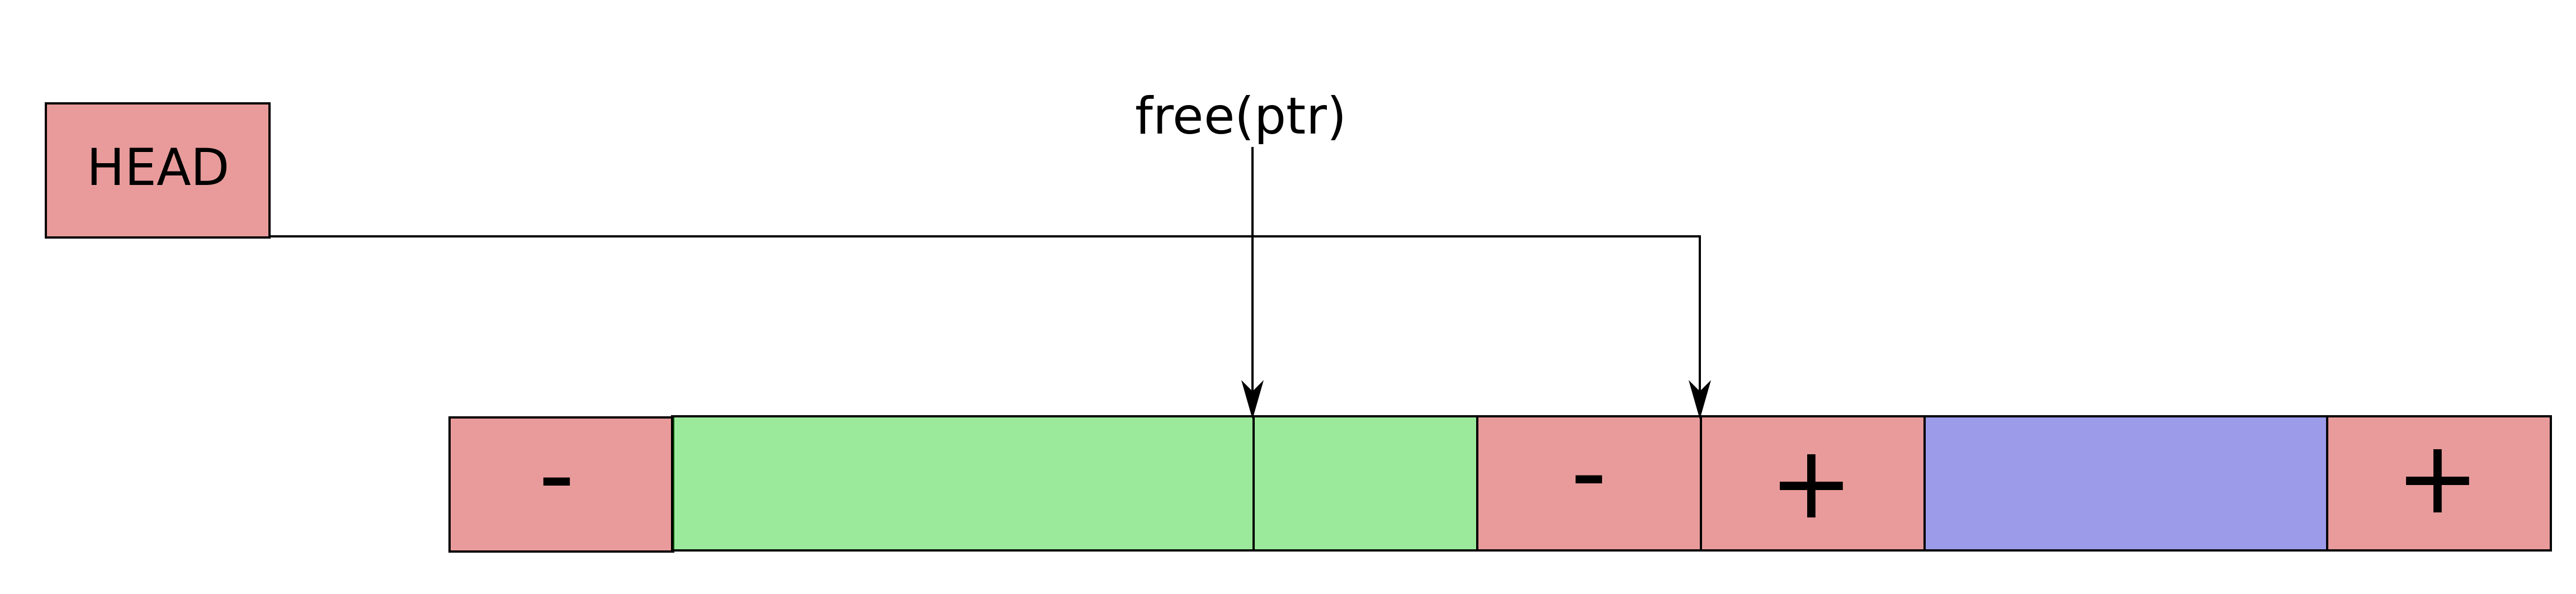
\includegraphics[height=.2\textheight]{lst7}
\end{frame}

\begin{frame}
\frametitle{Граничные маркеры}
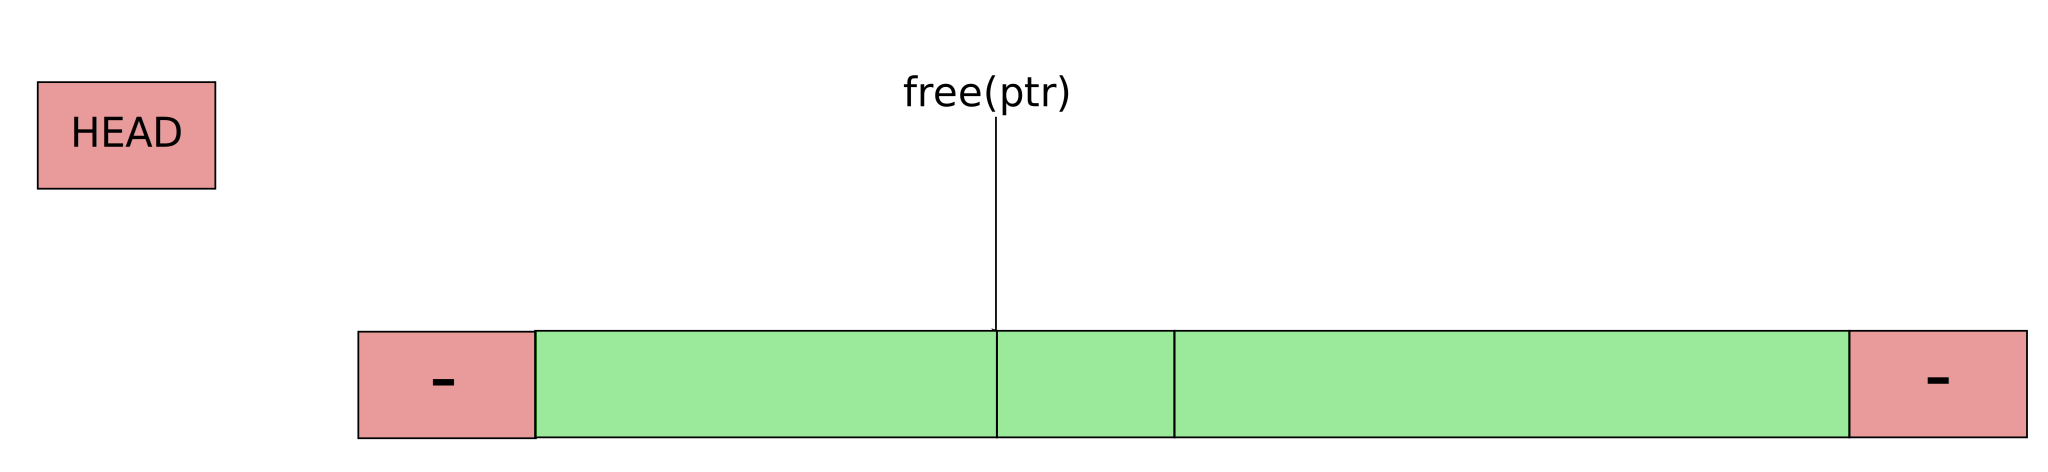
\includegraphics[height=.2\textheight]{lst8}
\end{frame}

\begin{frame}
\frametitle{Граничные маркеры}
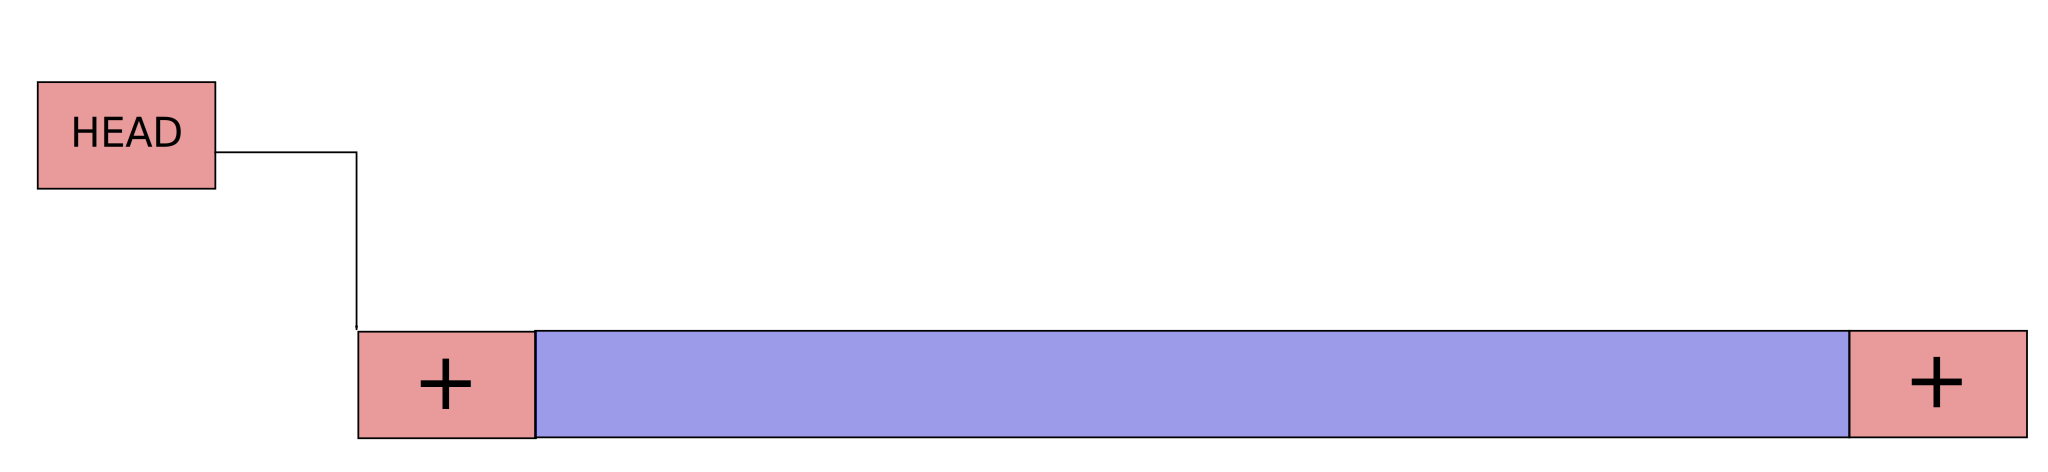
\includegraphics[height=.2\textheight]{lst9}
\end{frame}


  \begin{frame}
\frametitle{Buddy аллокатор}
\begin{itemize}
    \item<1->Buddy аллокатор предназначен для аллокации больших участков памяти
    \begin{itemize}
        \item<2->buddy аллокатор аллоцирует память блоками;
        \item<3->блок - $2^i$ последовательных страниц;
        \item<4->например, 1 страница, 2 страницы, 4 страницы и т. д.;
	\item<4->но не 3 страницы или 5 страниц.
    \end{itemize}
\end{itemize}
\end{frame}

\begin{frame}
\frametitle{Дескрипторы страниц}
\begin{itemize}
    \item<1->Buddy аллокатор не будет работать с памятью напрямую
    \begin{itemize}
        \item<2->вместо страниц памяти будем использовать в алгоритме
        дескрипторы;
        \item<3->просто массив дескрипторов - по адресу страницы легко получить
        дескриптор и наоборот.
    \end{itemize}
\end{itemize}
\end{frame}

\begin{frame}
\frametitle{Дескрипторы страниц}
\begin{itemize}
    \item<1->Что будет храниться в дескрипторах?
    \begin{itemize}
        \item<2->указатели, чтобы связать дескрипторы в двусвязный список;
        \item<3->признак свободности/занятости;
        \item<4->уровень (указание на размер блока).
    \end{itemize}
\end{itemize}
\end{frame}

\begin{frame}
\frametitle{Списки свободных блоков}
\begin{itemize}
    \item<1->Пусть у нас изначально есть $2^N$ последовательных свободных
    страниц:
    \begin{itemize}
        \item<1->заведем $N + 1$ изначально пустой двусвязный список;
        \item<1->$i$-ый список будет хранить свободные блоки размером $2^i$
        страниц.
    \end{itemize}
\end{itemize}
\end{frame}

\begin{frame}
\frametitle{Начальное состояние}
\begin{itemize}
    \item<1->Возьмем дескриптор $0$-ой страницы
    \begin{itemize}
        \item<2->отметим дескриптор как свободный;
        \item<3->зададим в дескрипторе уровень $N-1$;
        \item<4->добавим дескриптор в список $N-1$.
    \end{itemize}
\end{itemize}
\end{frame}

\begin{frame}
\frametitle{Инициализация}
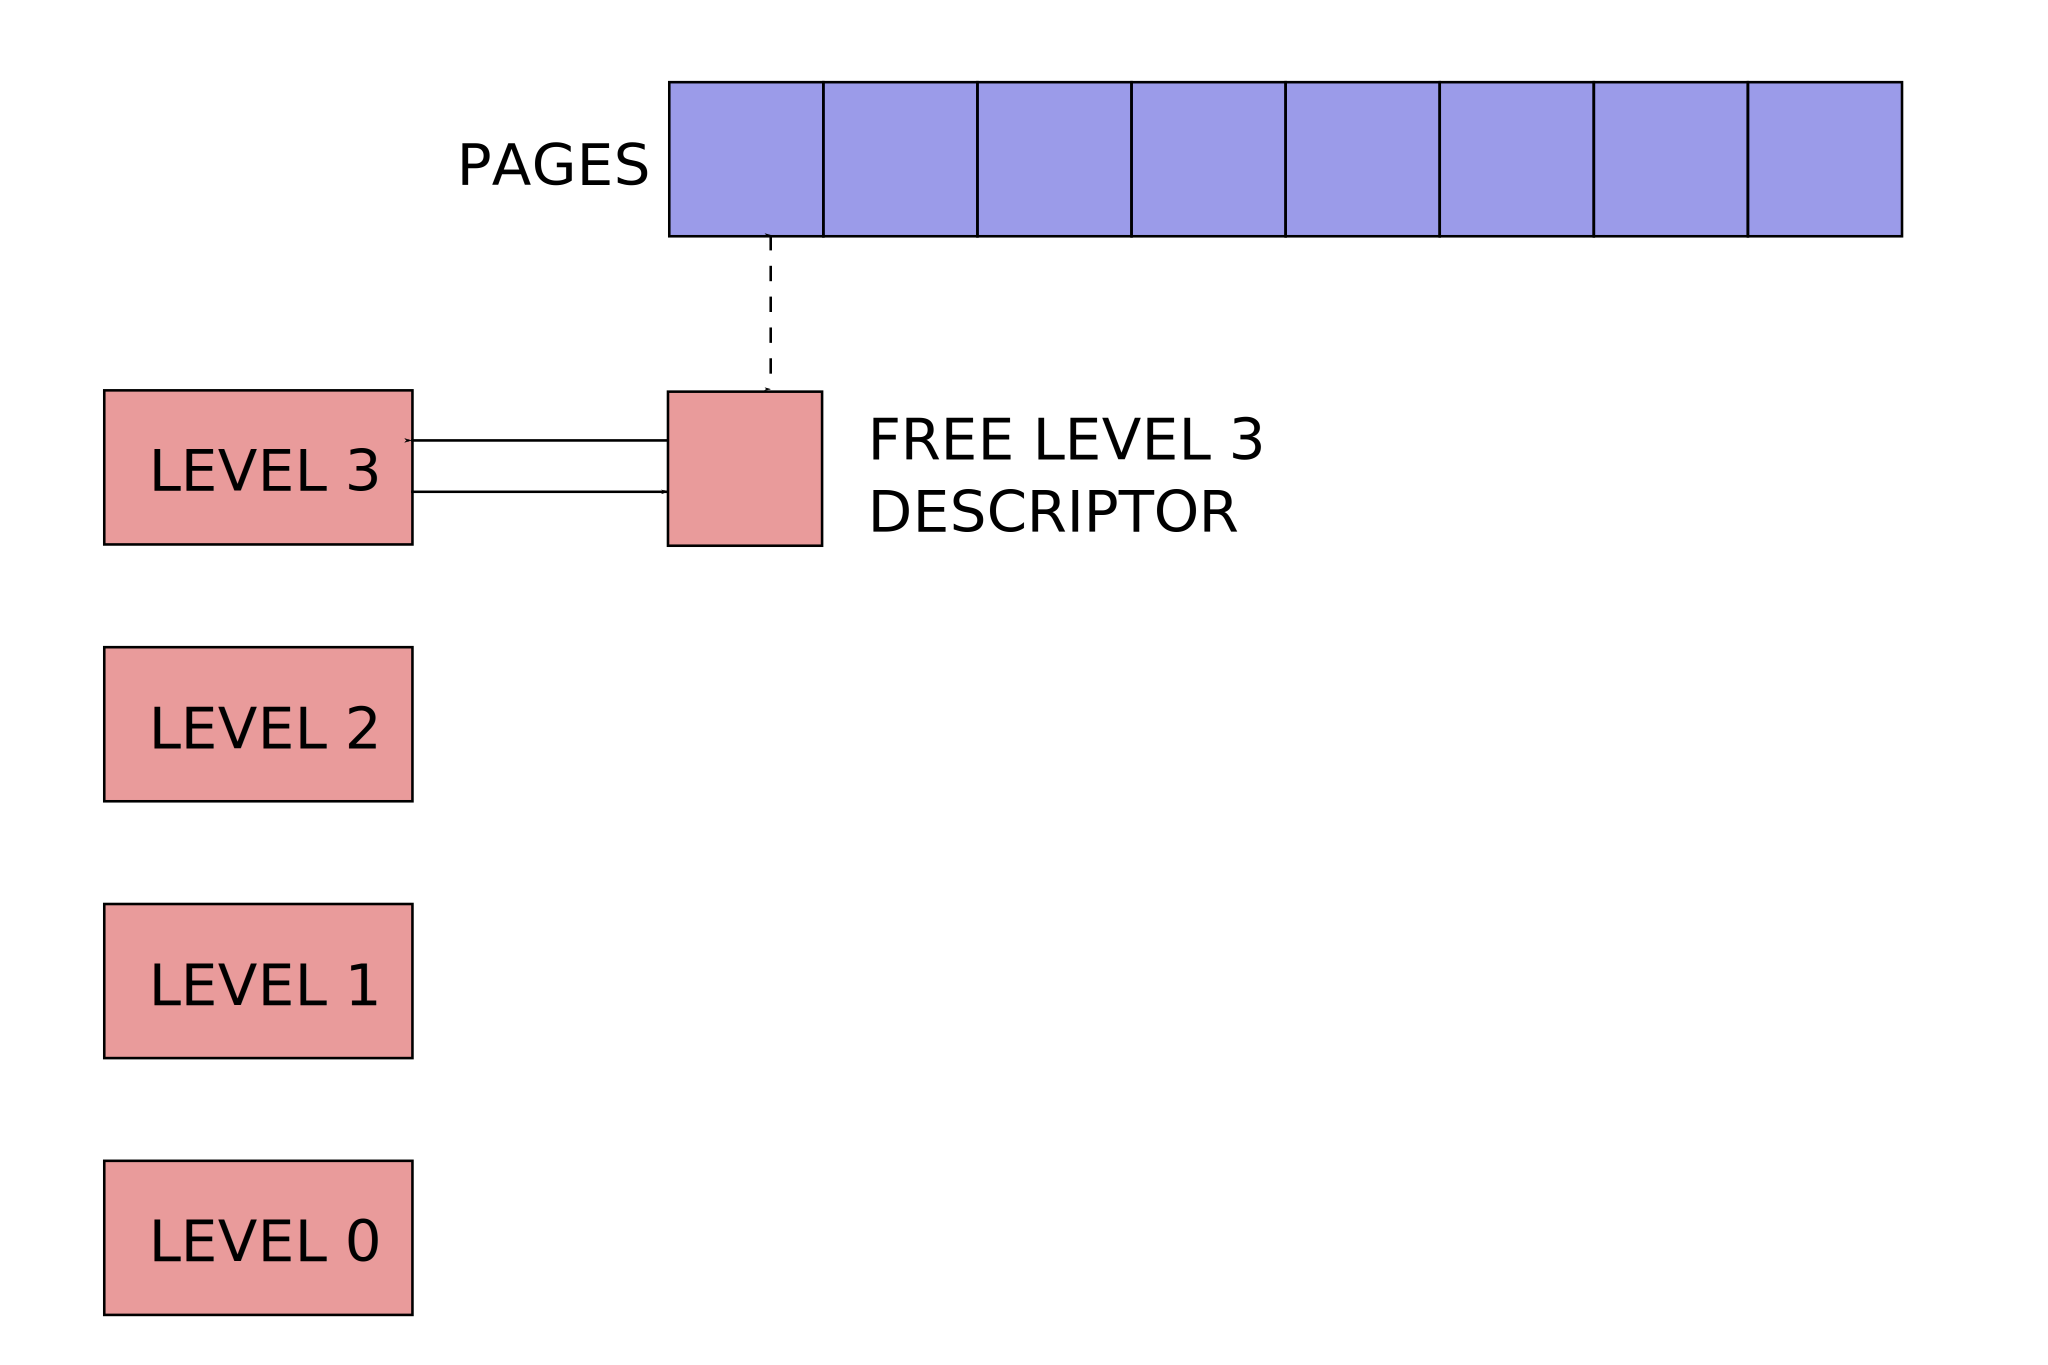
\includegraphics[height=.43\textheight]{bud0}
\end{frame}

\begin{frame}
\frametitle{Аллокация}
\begin{itemize}
    \item<1->Мы хотим аллоцировать $2^i$ страниц
    \begin{itemize}
        \item<2->найдем непустой список с блоками $\ge 2^i$;
        \item<3->берем один из блоков и делим его пополам, пока не останется
        $2^i$.
    \end{itemize}
\end{itemize}
\end{frame}

\begin{frame}
\frametitle{Аллокация}
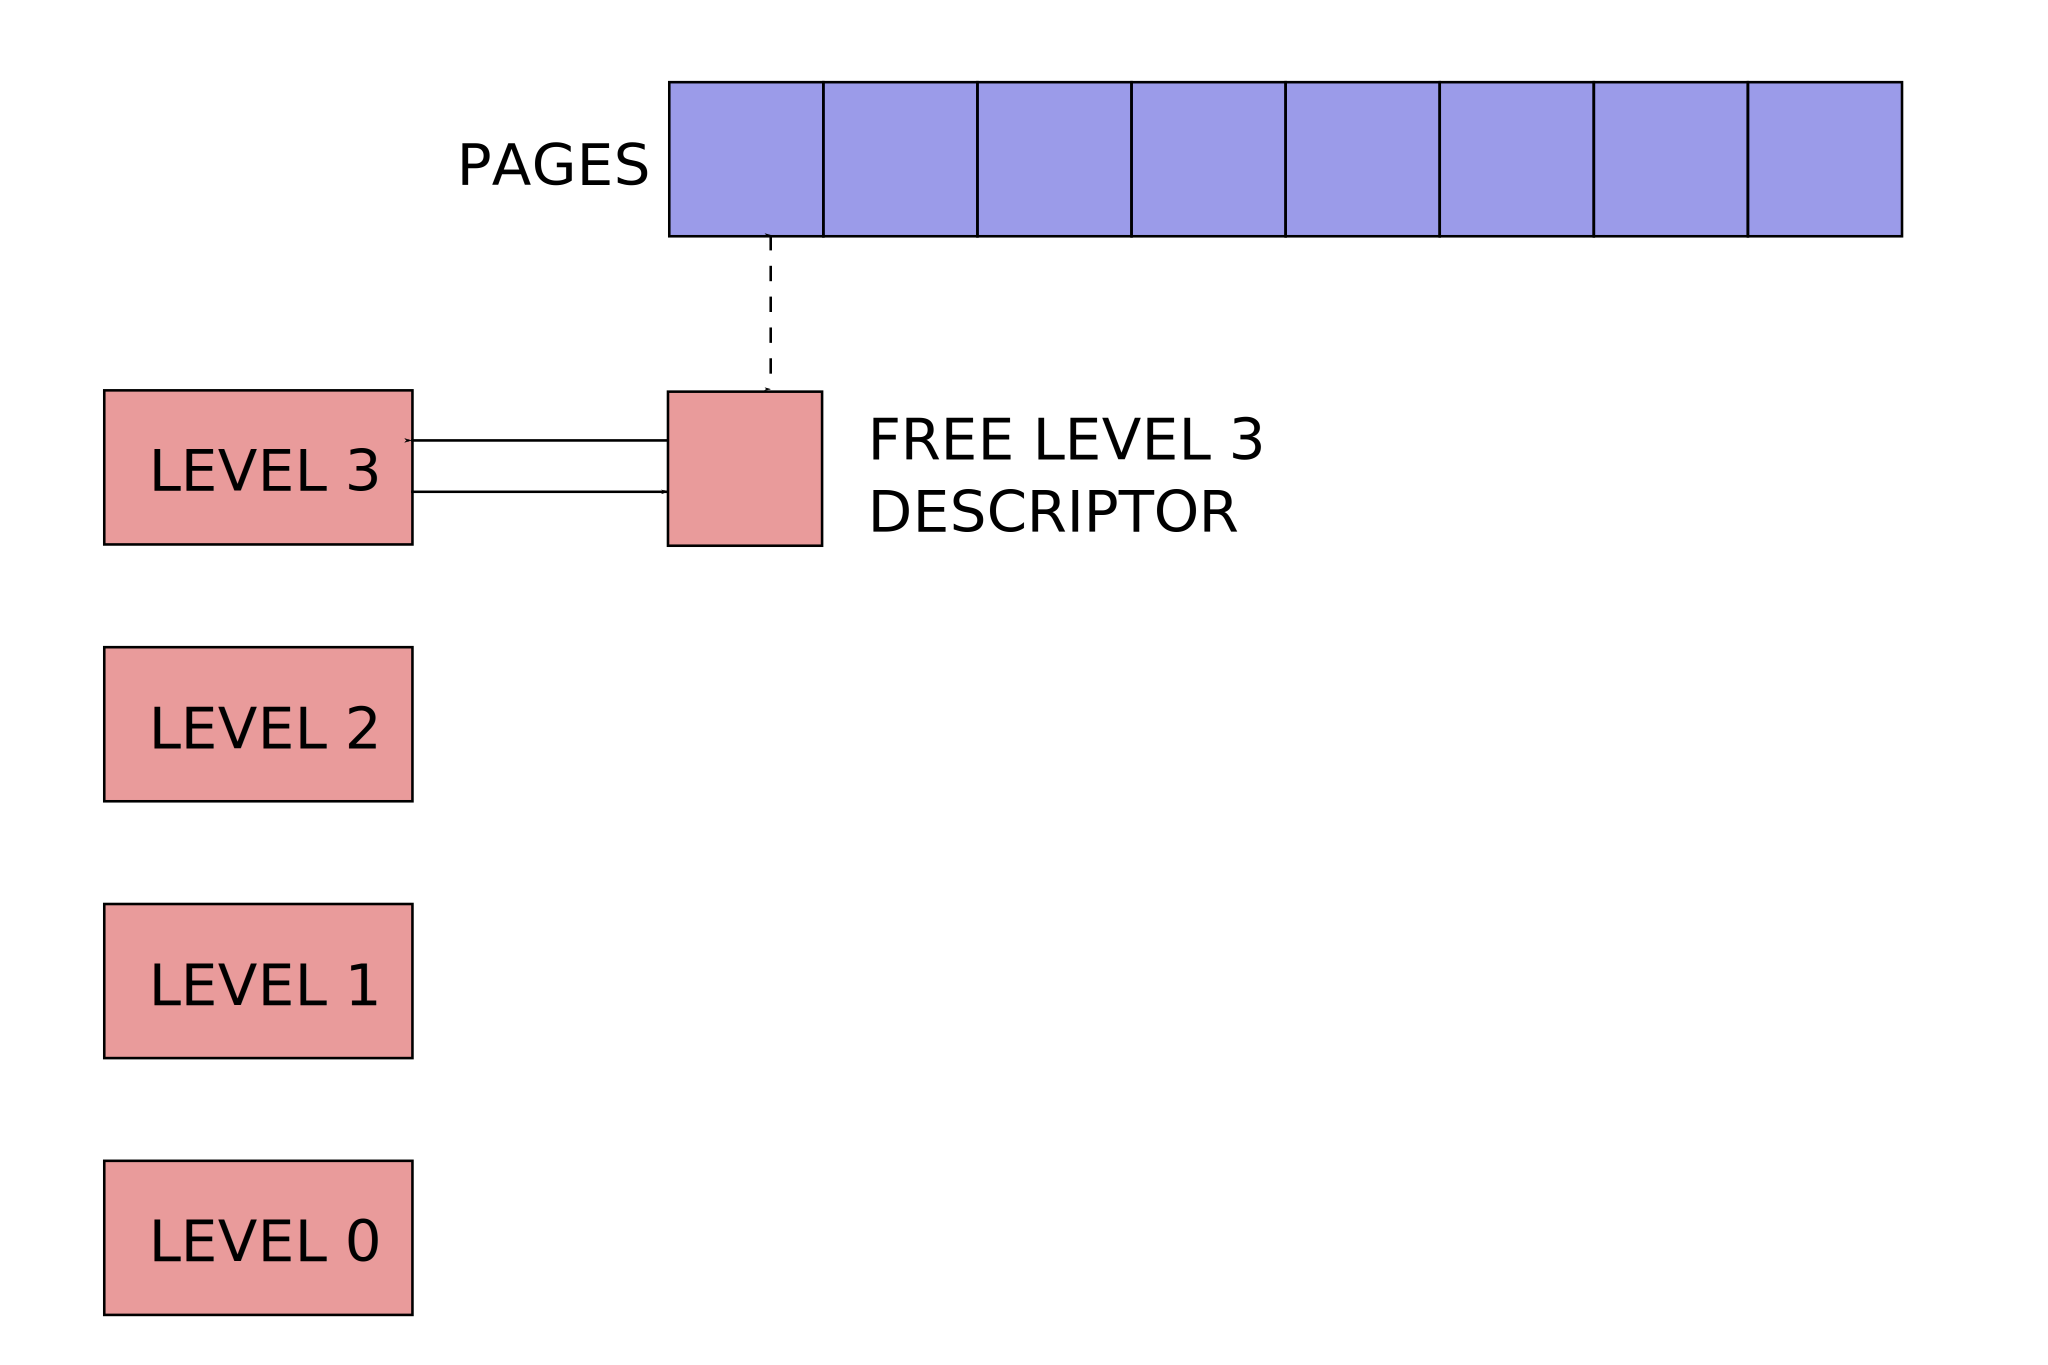
\includegraphics[height=.43\textheight]{bud0}
\end{frame}

\begin{frame}
\frametitle{Аллокация}
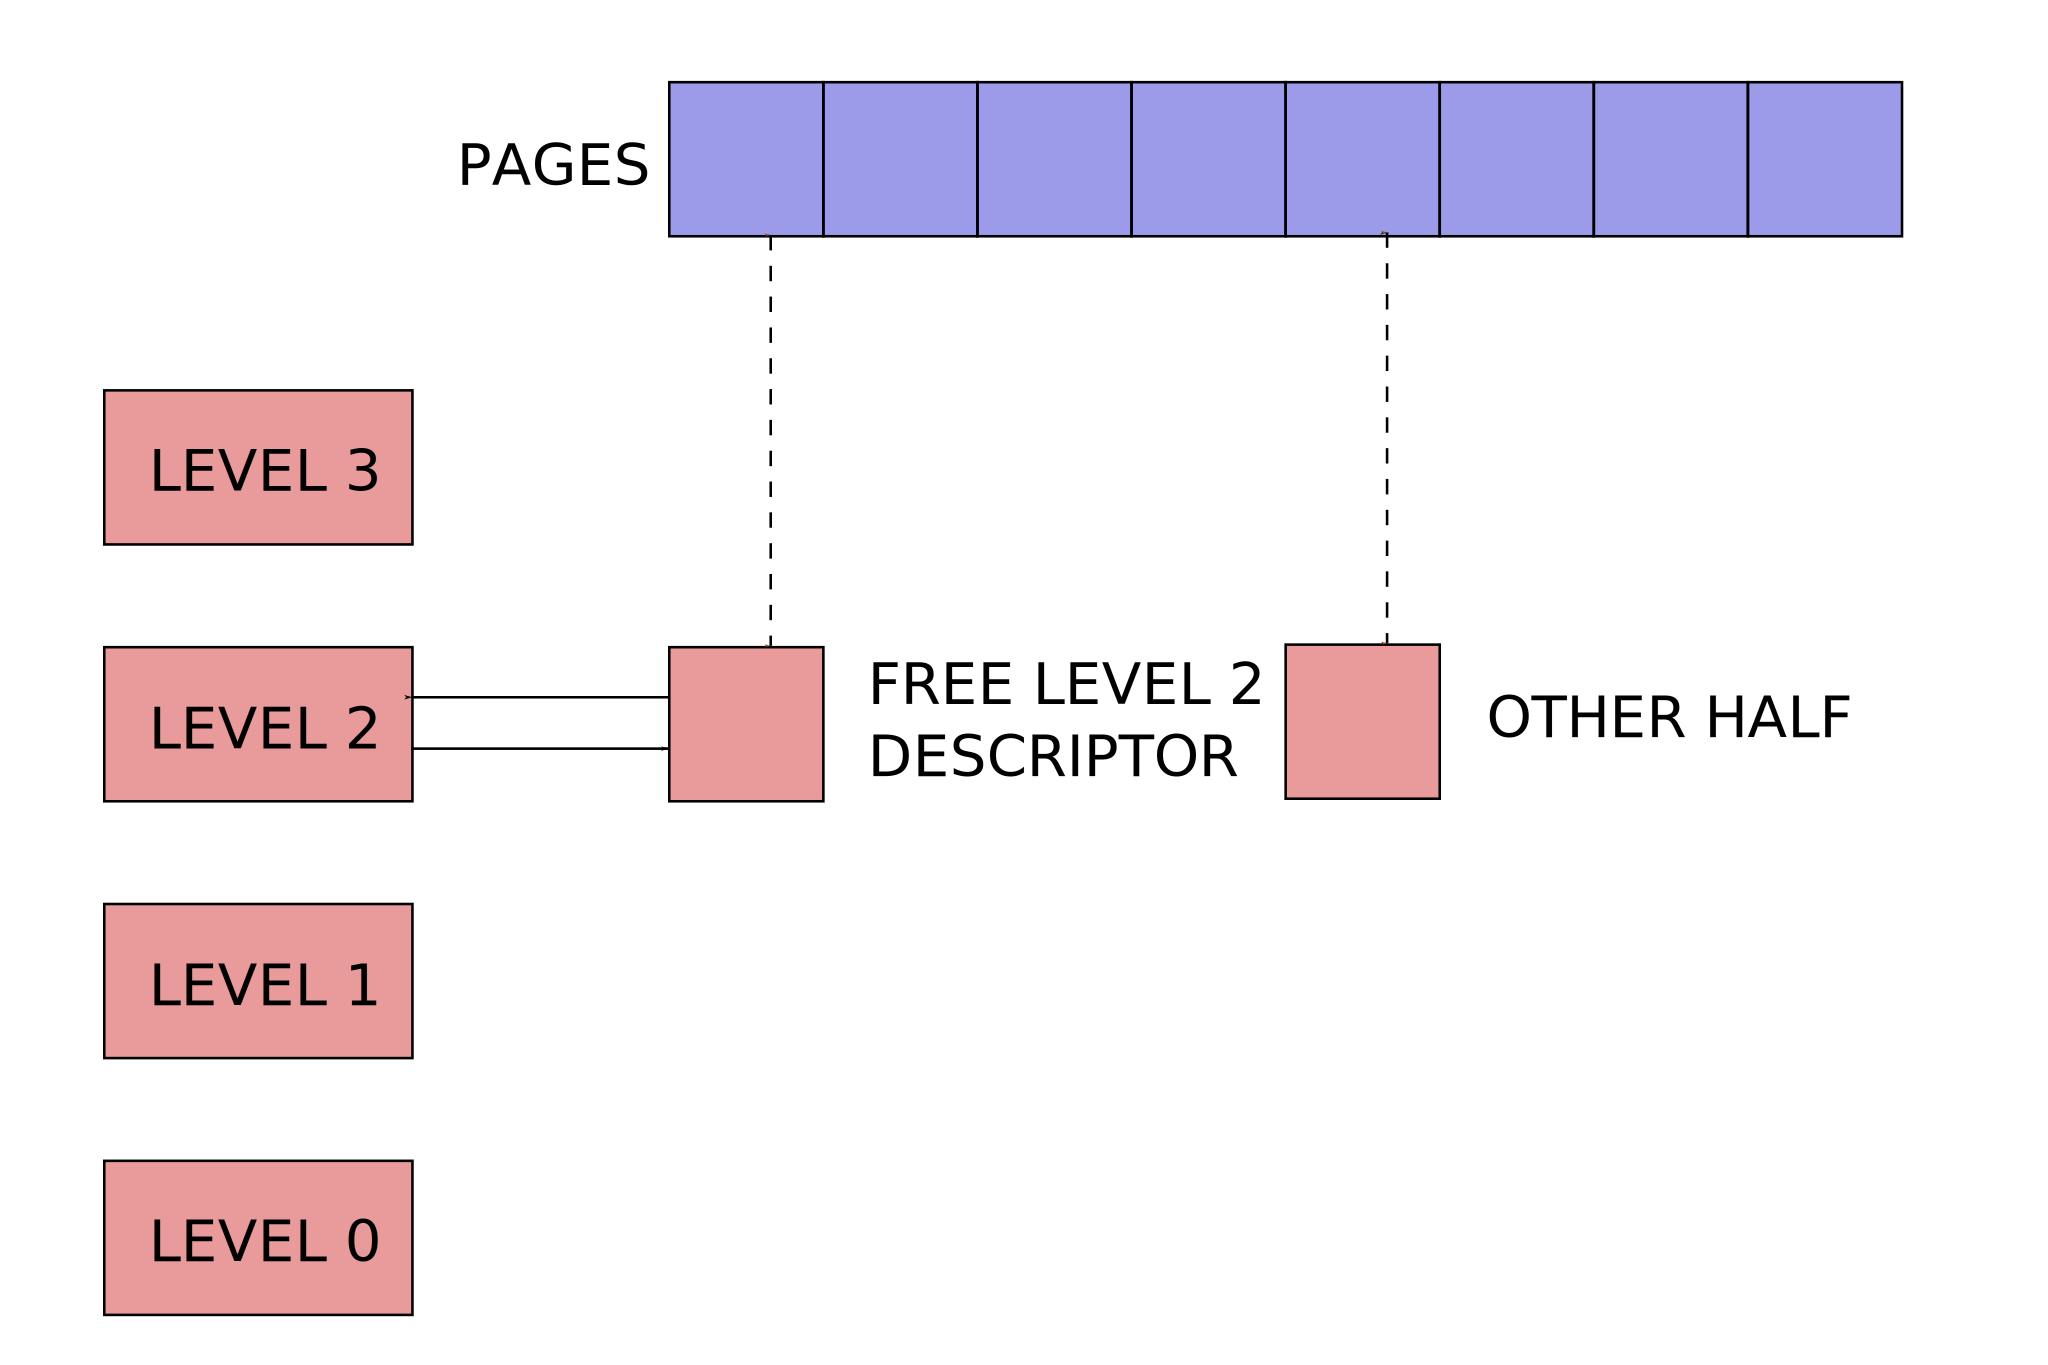
\includegraphics[height=.43\textheight]{bud1}
\end{frame}

\begin{frame}
\frametitle{Аллокация}
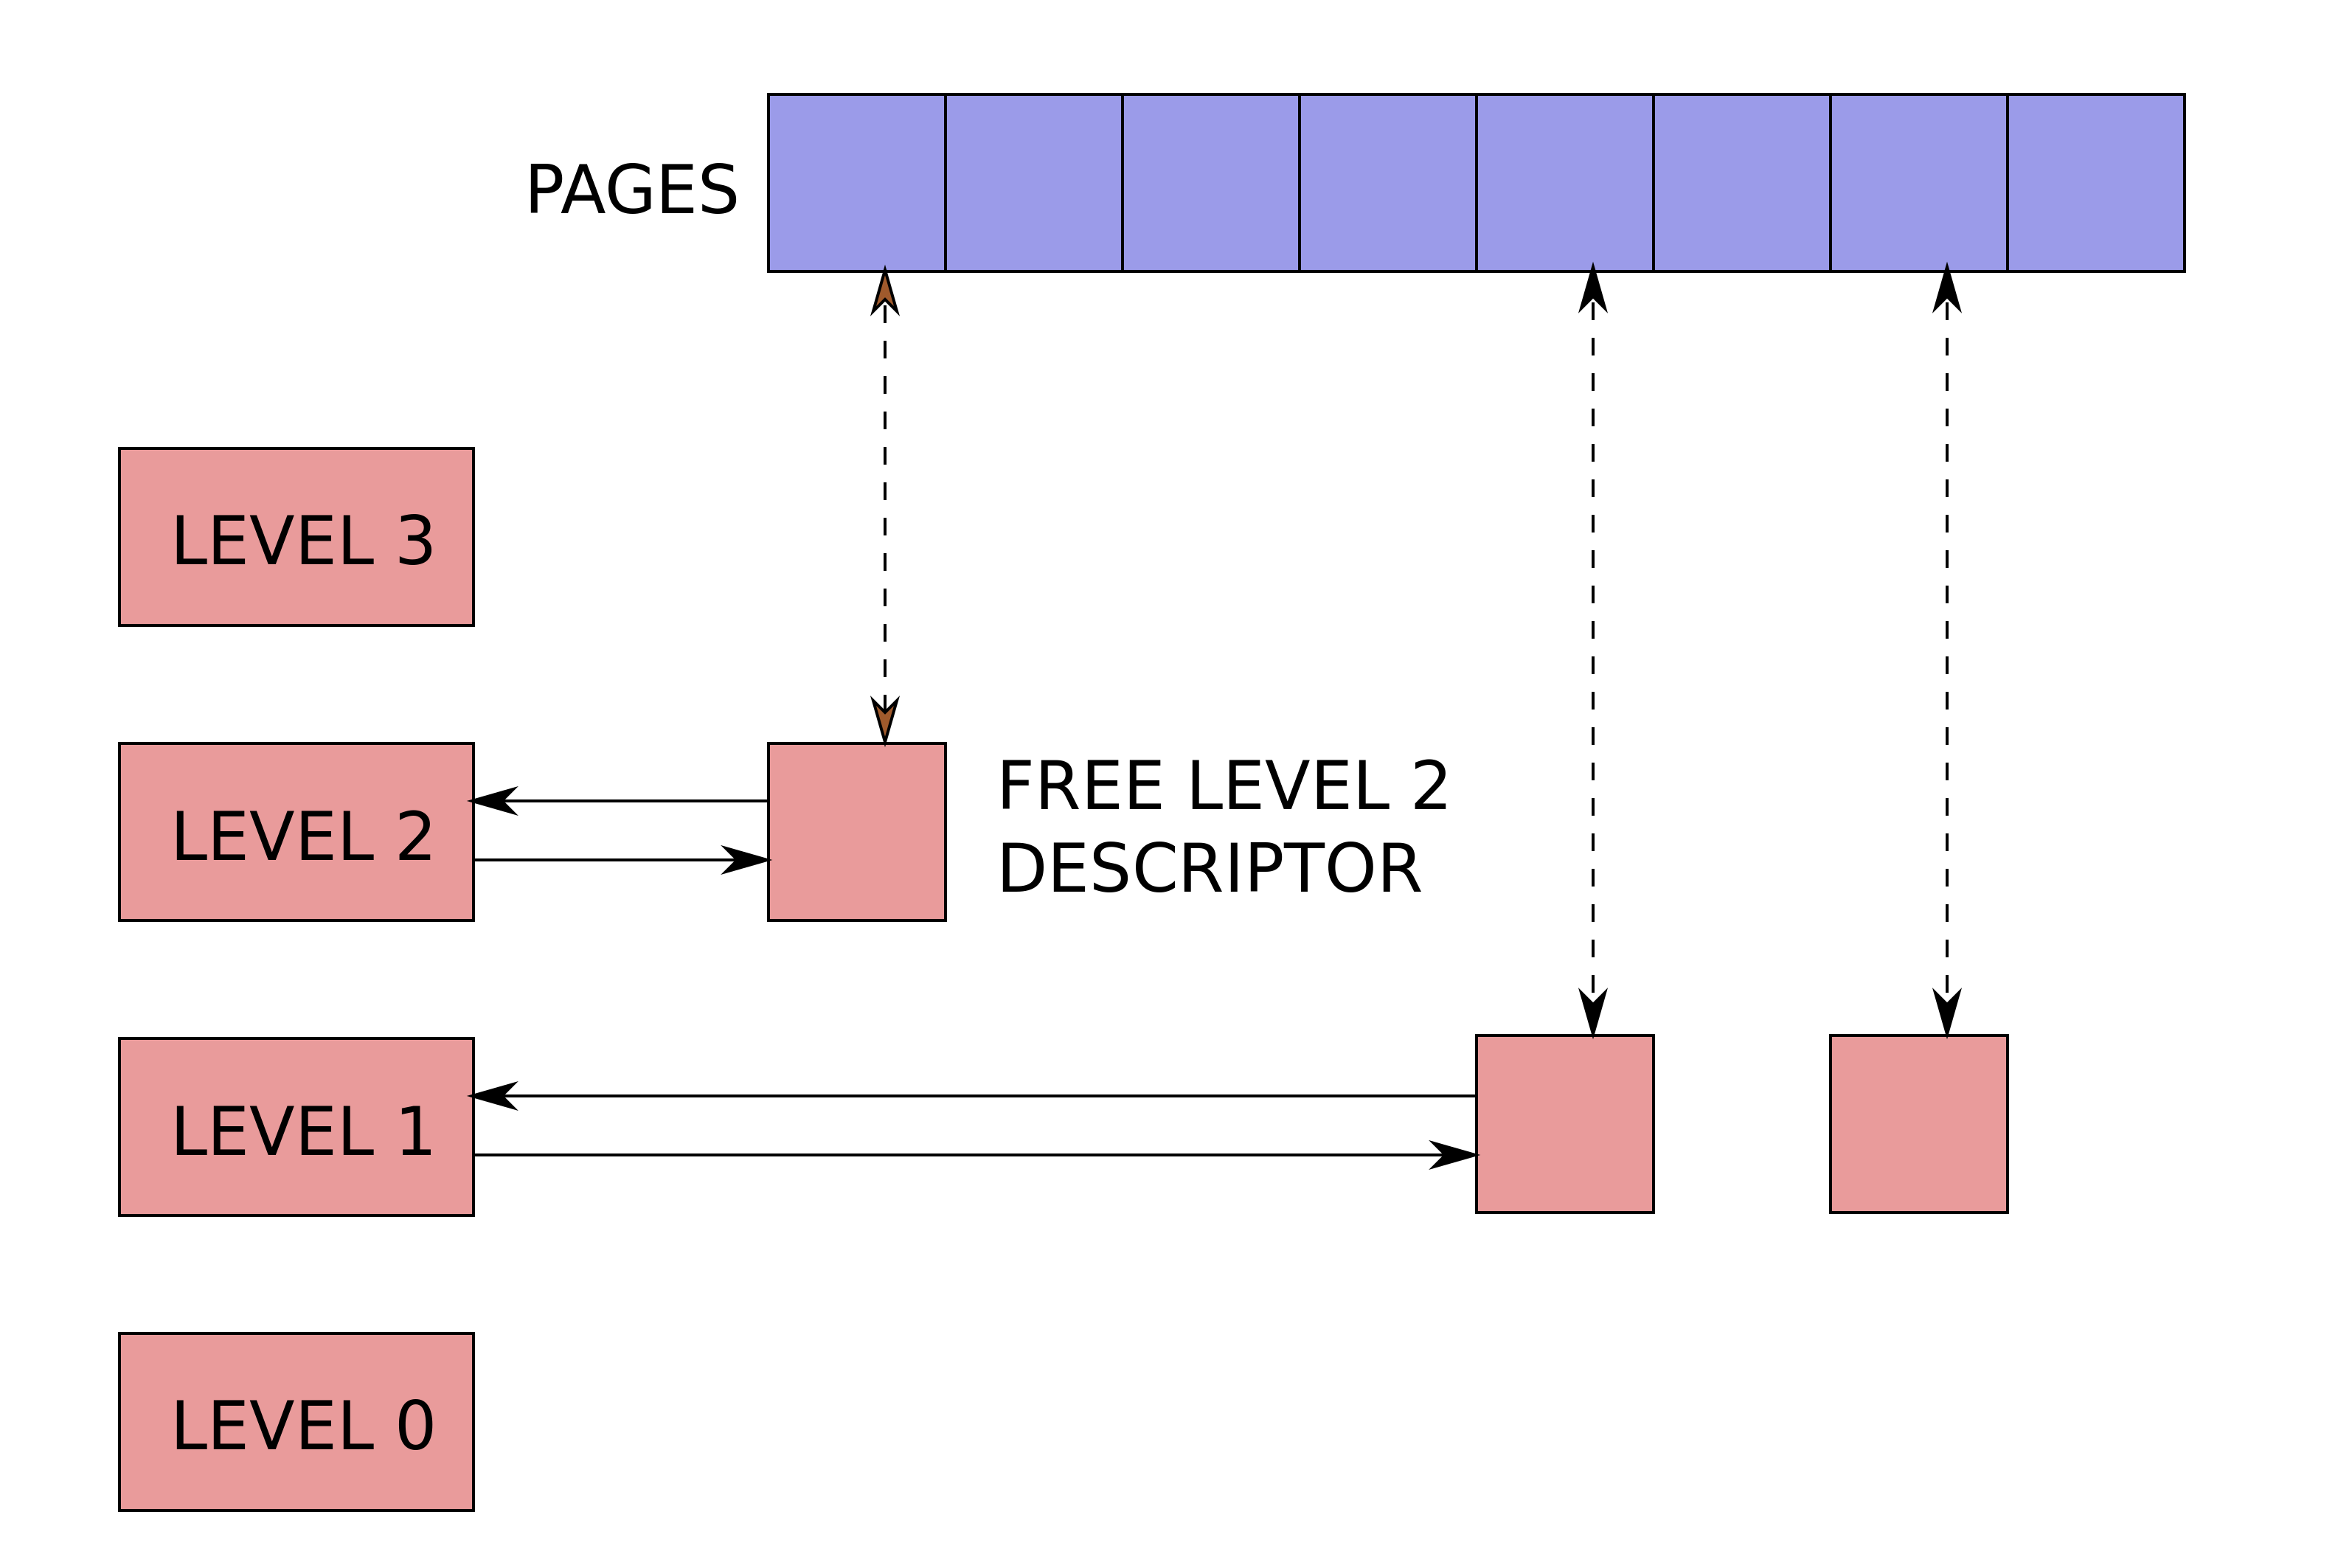
\includegraphics[height=.43\textheight]{bud2}
\end{frame}

\begin{frame}
\frametitle{Аллокация}
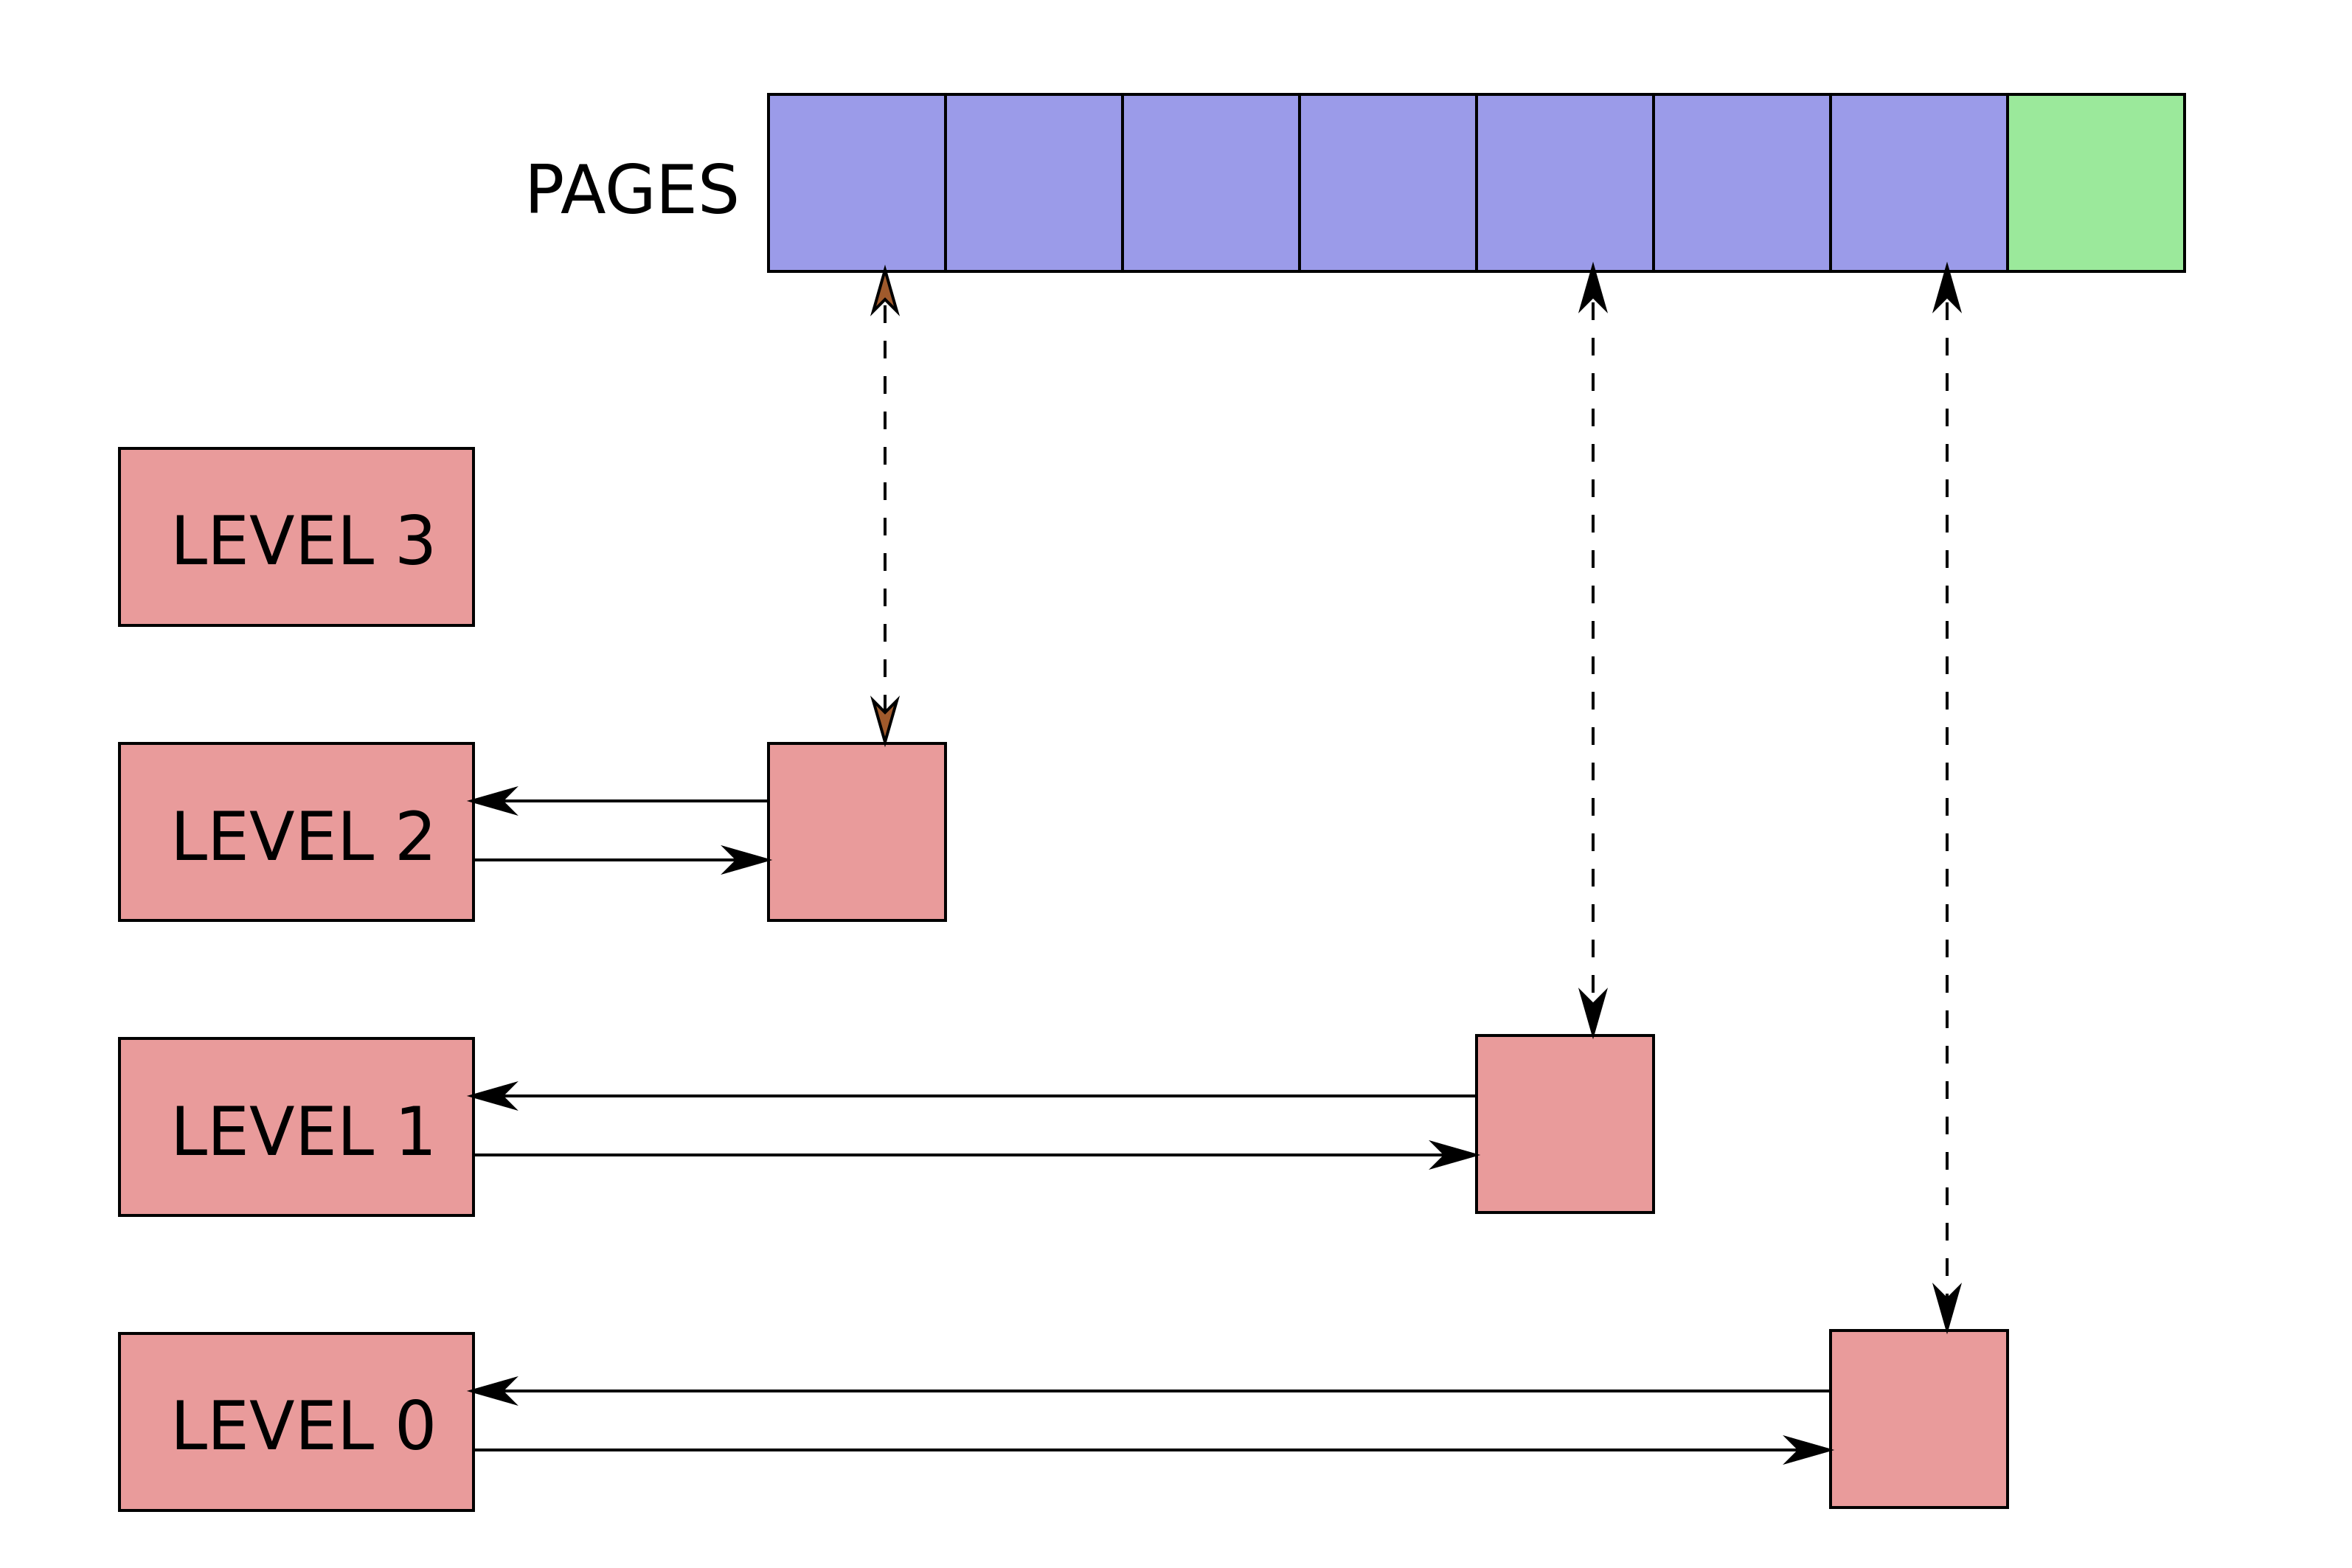
\includegraphics[height=.43\textheight]{bud3}
\end{frame}

\begin{frame}
\frametitle{Освобождение}
\begin{itemize}
    \item<1->Теперь мы хотим освободить блок размера $2^i$
    \begin{itemize}
        \item<2->мы могли бы просто добавить дескриптор в список $i$, но это
        приведет к фрагментации;
        \item<3->мы должны попытаться объединить смежные блоки.
    \end{itemize}
\end{itemize}
\end{frame}

\begin{frame}
\frametitle{Buddies}
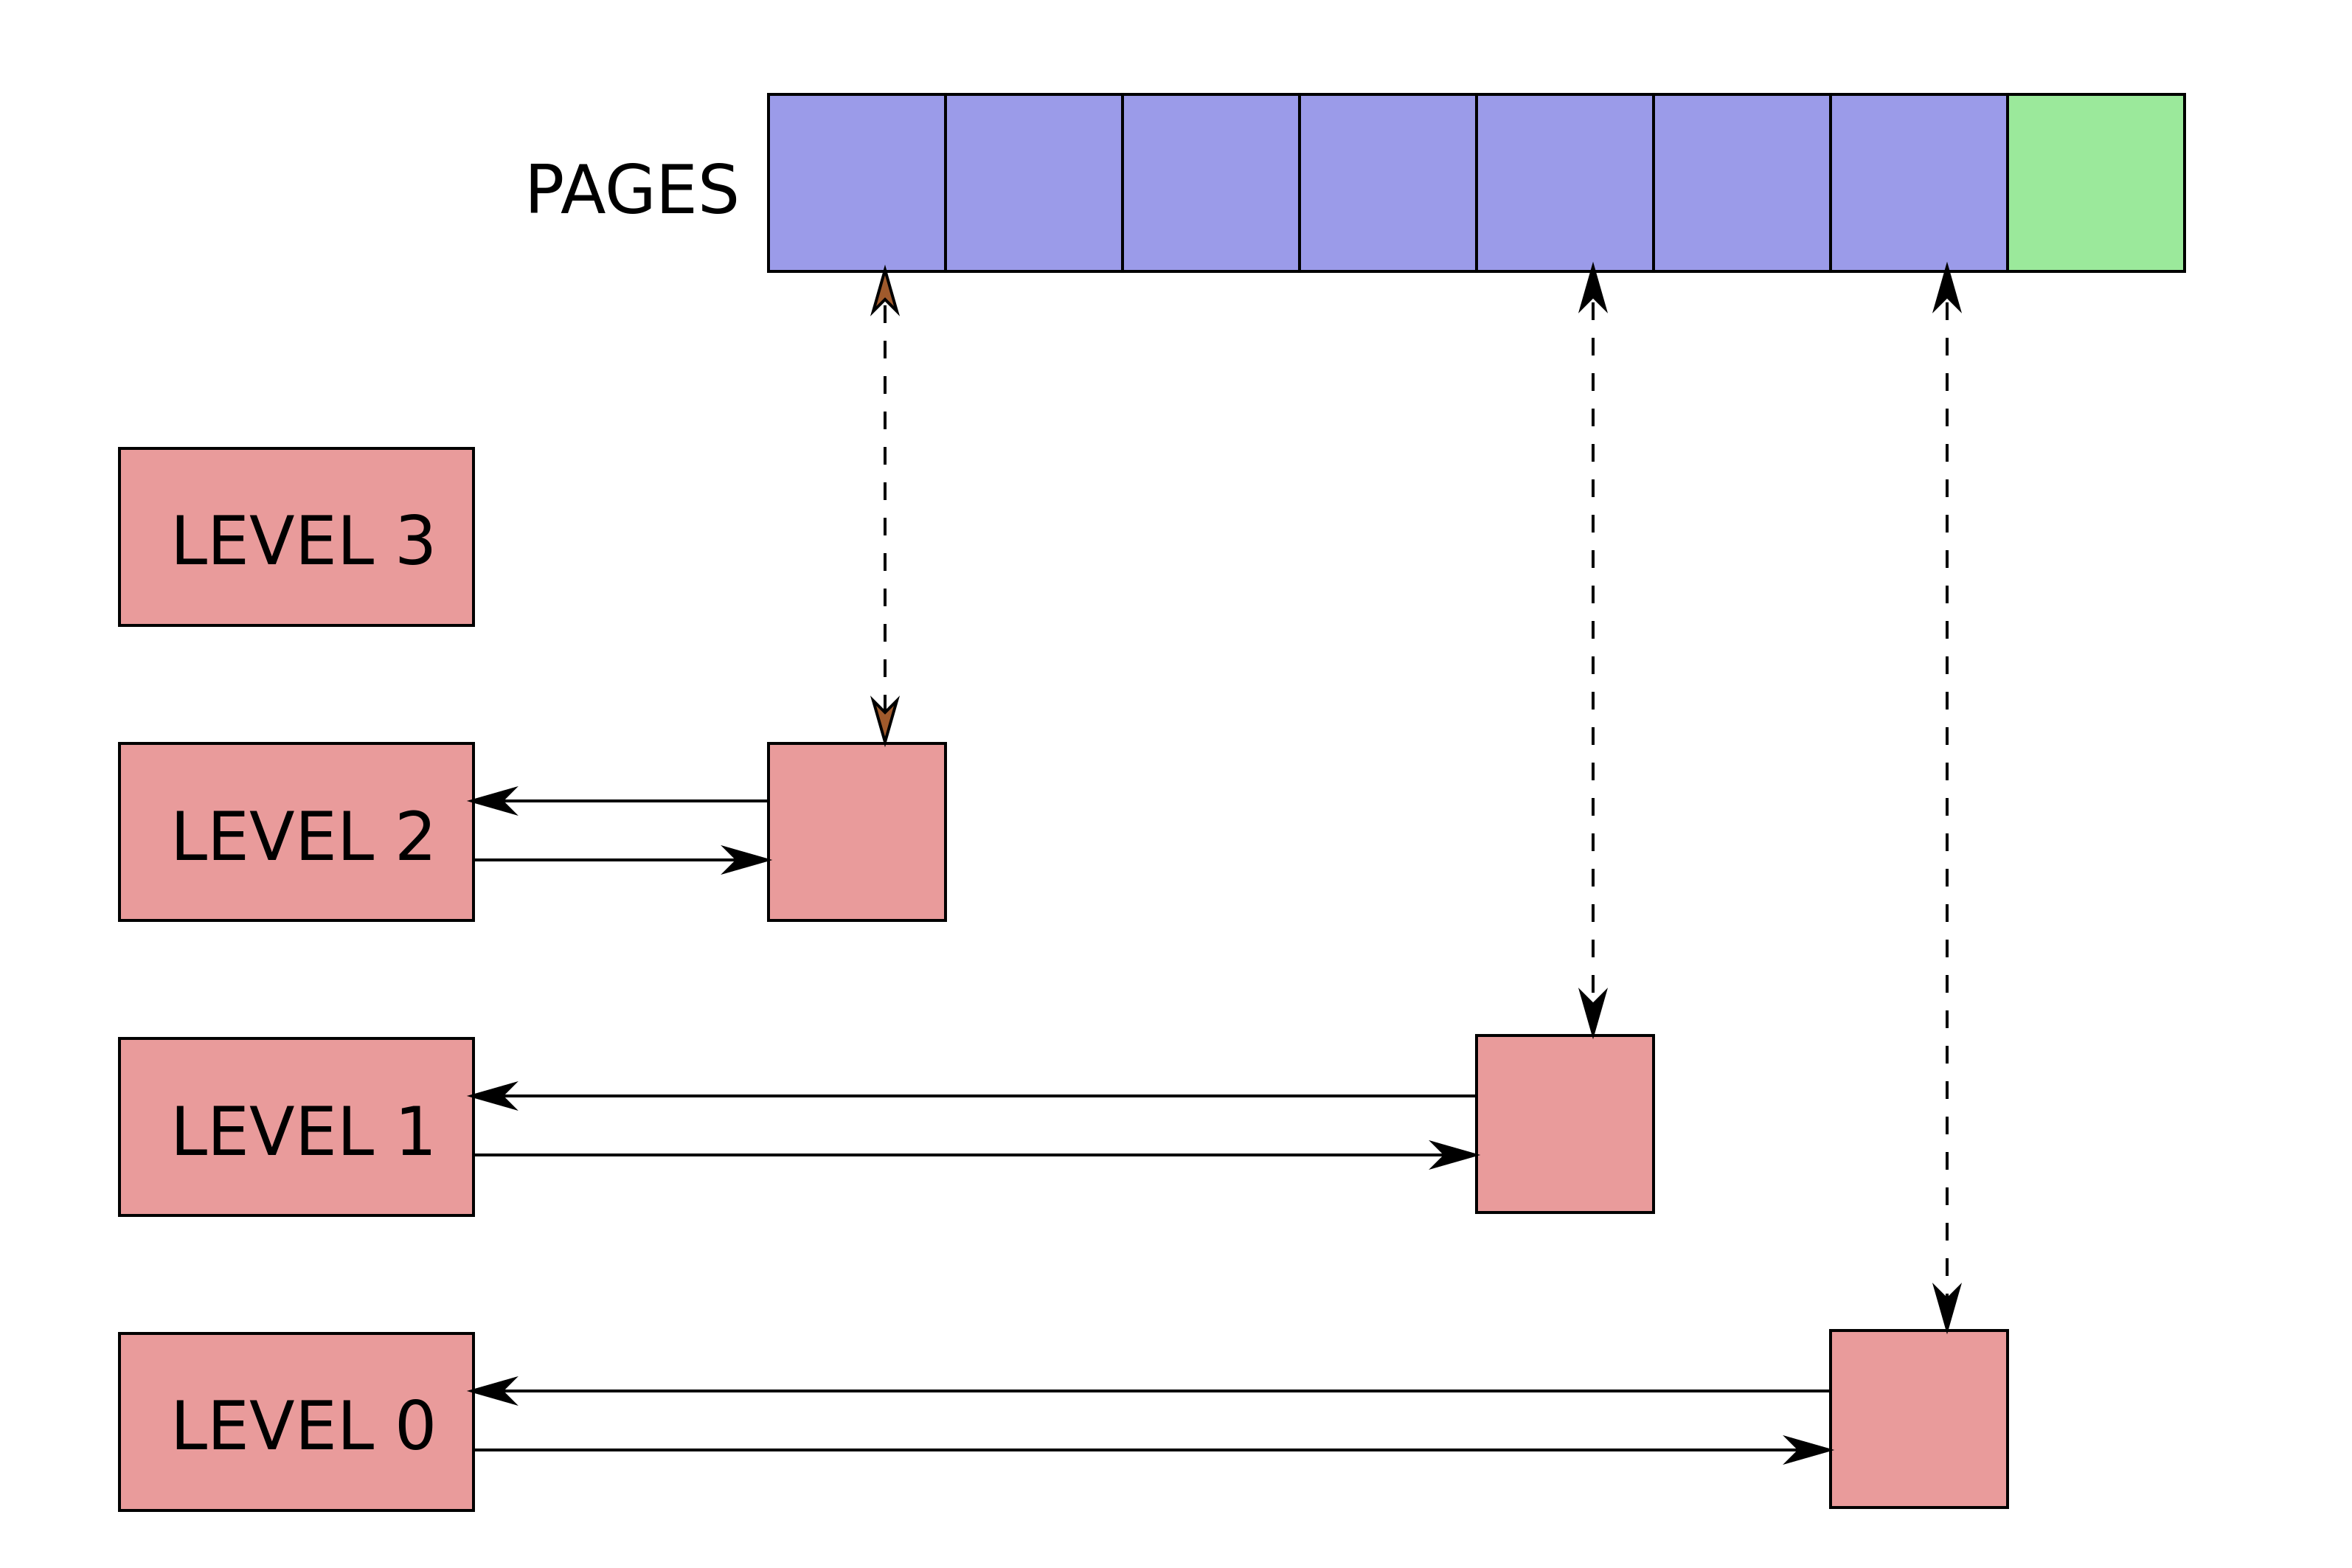
\includegraphics[height=.43\textheight]{bud3}
\end{frame}

\begin{frame}
\frametitle{Buddies}
\begin{itemize}
    \item<1->Как найти парный блок?
    \begin{itemize}
        \item<1->если мы осовобождаем блок размера $2^i$ с номером $j$;
        \item<2->парный блок имеет номер $j \oplus 2^i$;
	\item<2->$\oplus$ - исключющее побитовое ИЛИ.
    \end{itemize}
\end{itemize}
\end{frame}

\begin{frame}
\frametitle{Освобождение}
\begin{itemize}
    \item<1->Когда можно объединять парные блоки?
    \begin{itemize}
        \item<2->если оба блока свободны;
        \item<3->если оба блока имеют один размер (уровень в дескрипторе).
    \end{itemize}
\end{itemize}
\end{frame}

\begin{frame}
\frametitle{Освбождение}
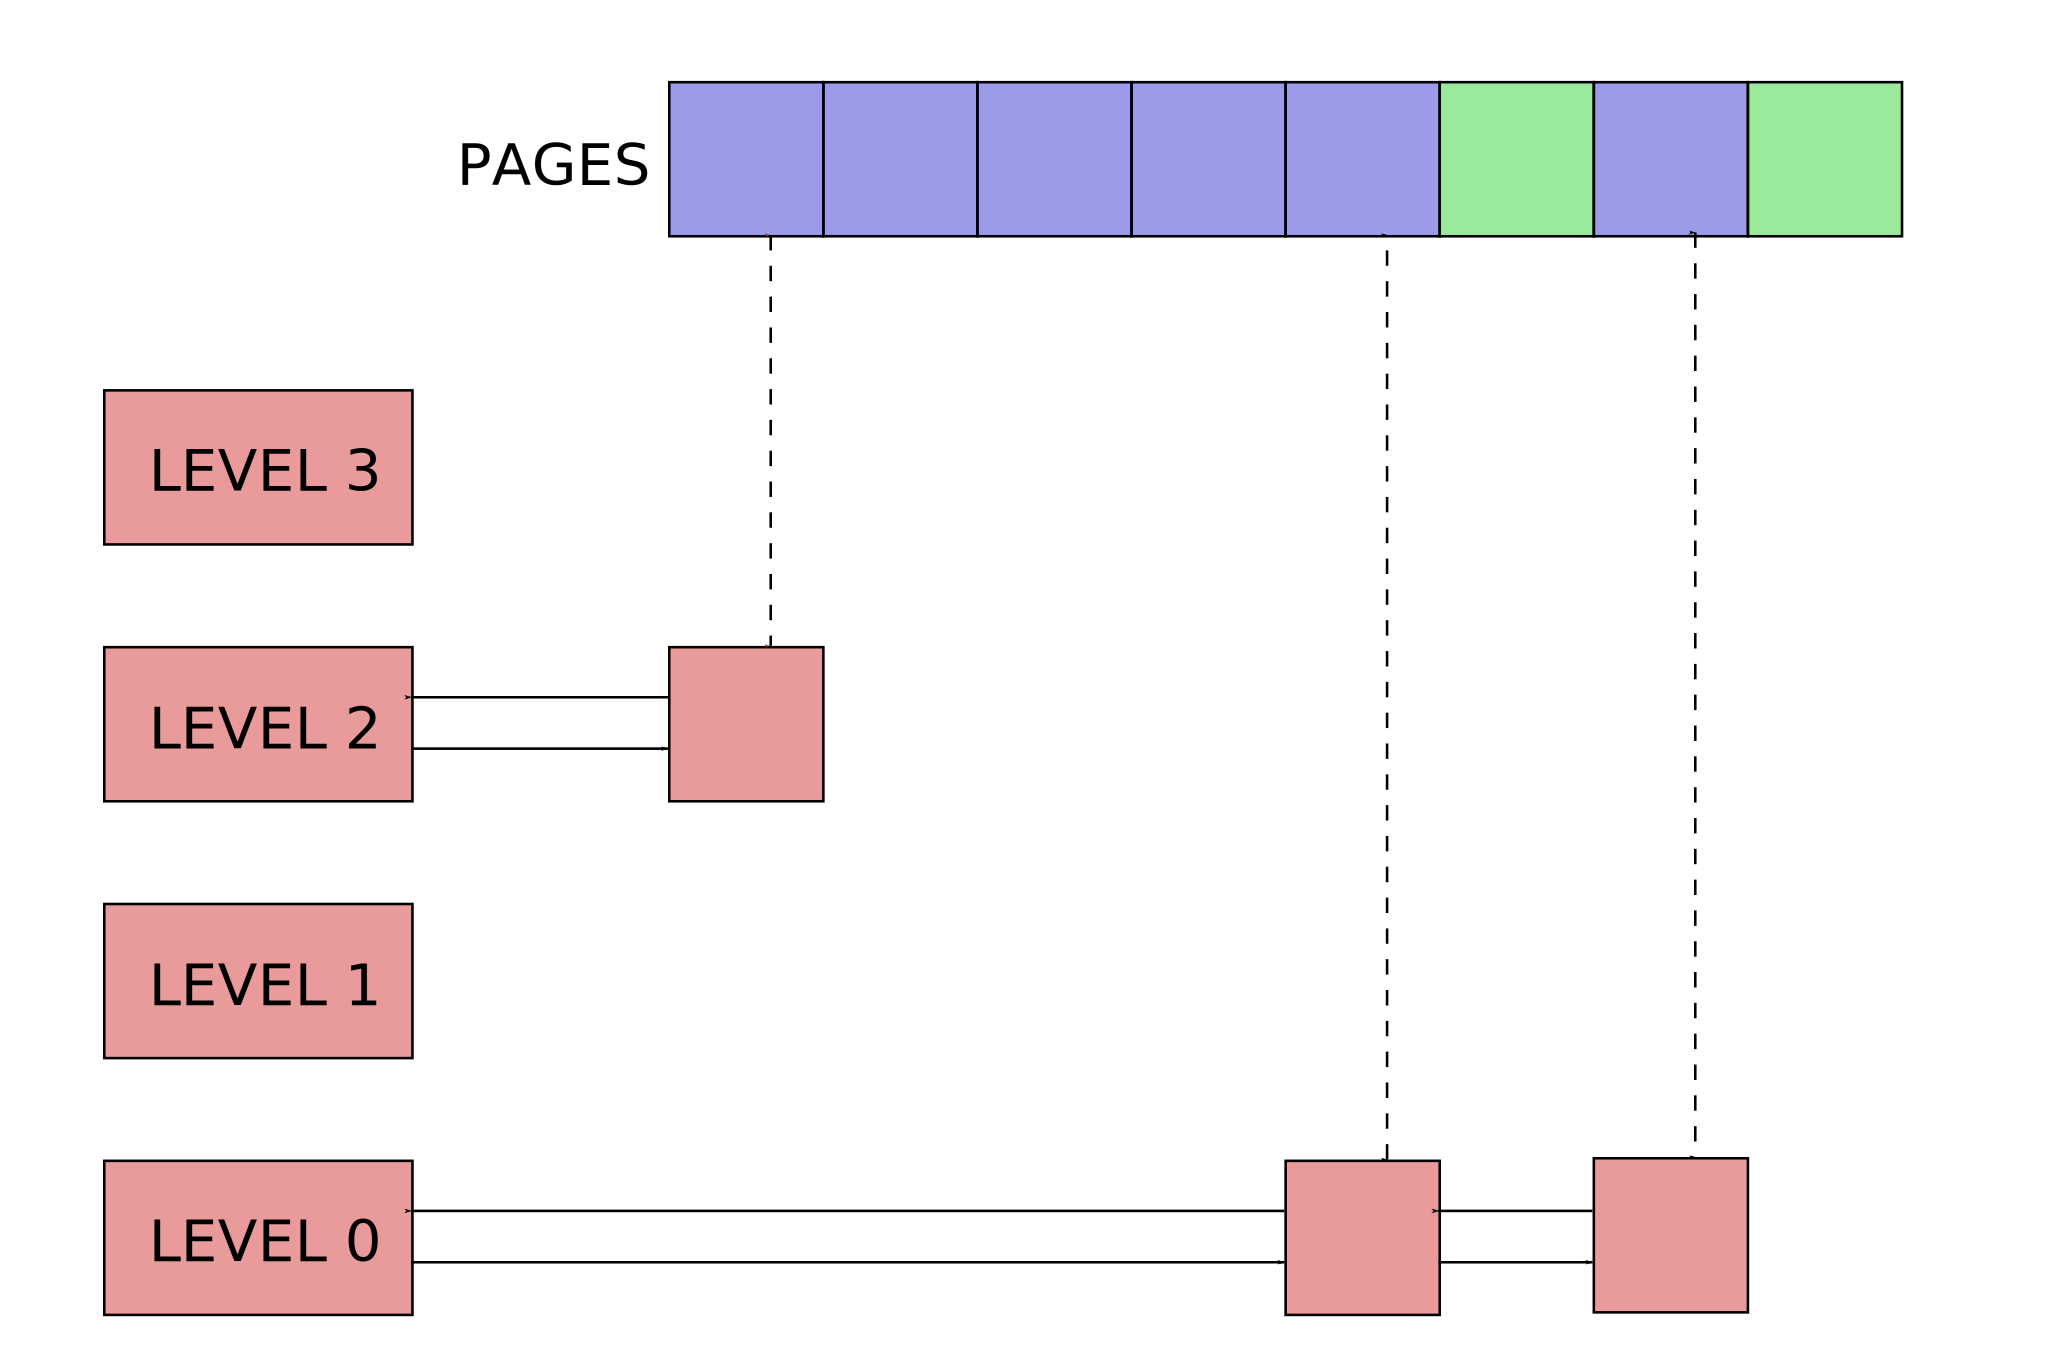
\includegraphics[height=.43\textheight]{bud4}
\end{frame}

\begin{frame}
\frametitle{Buddies}
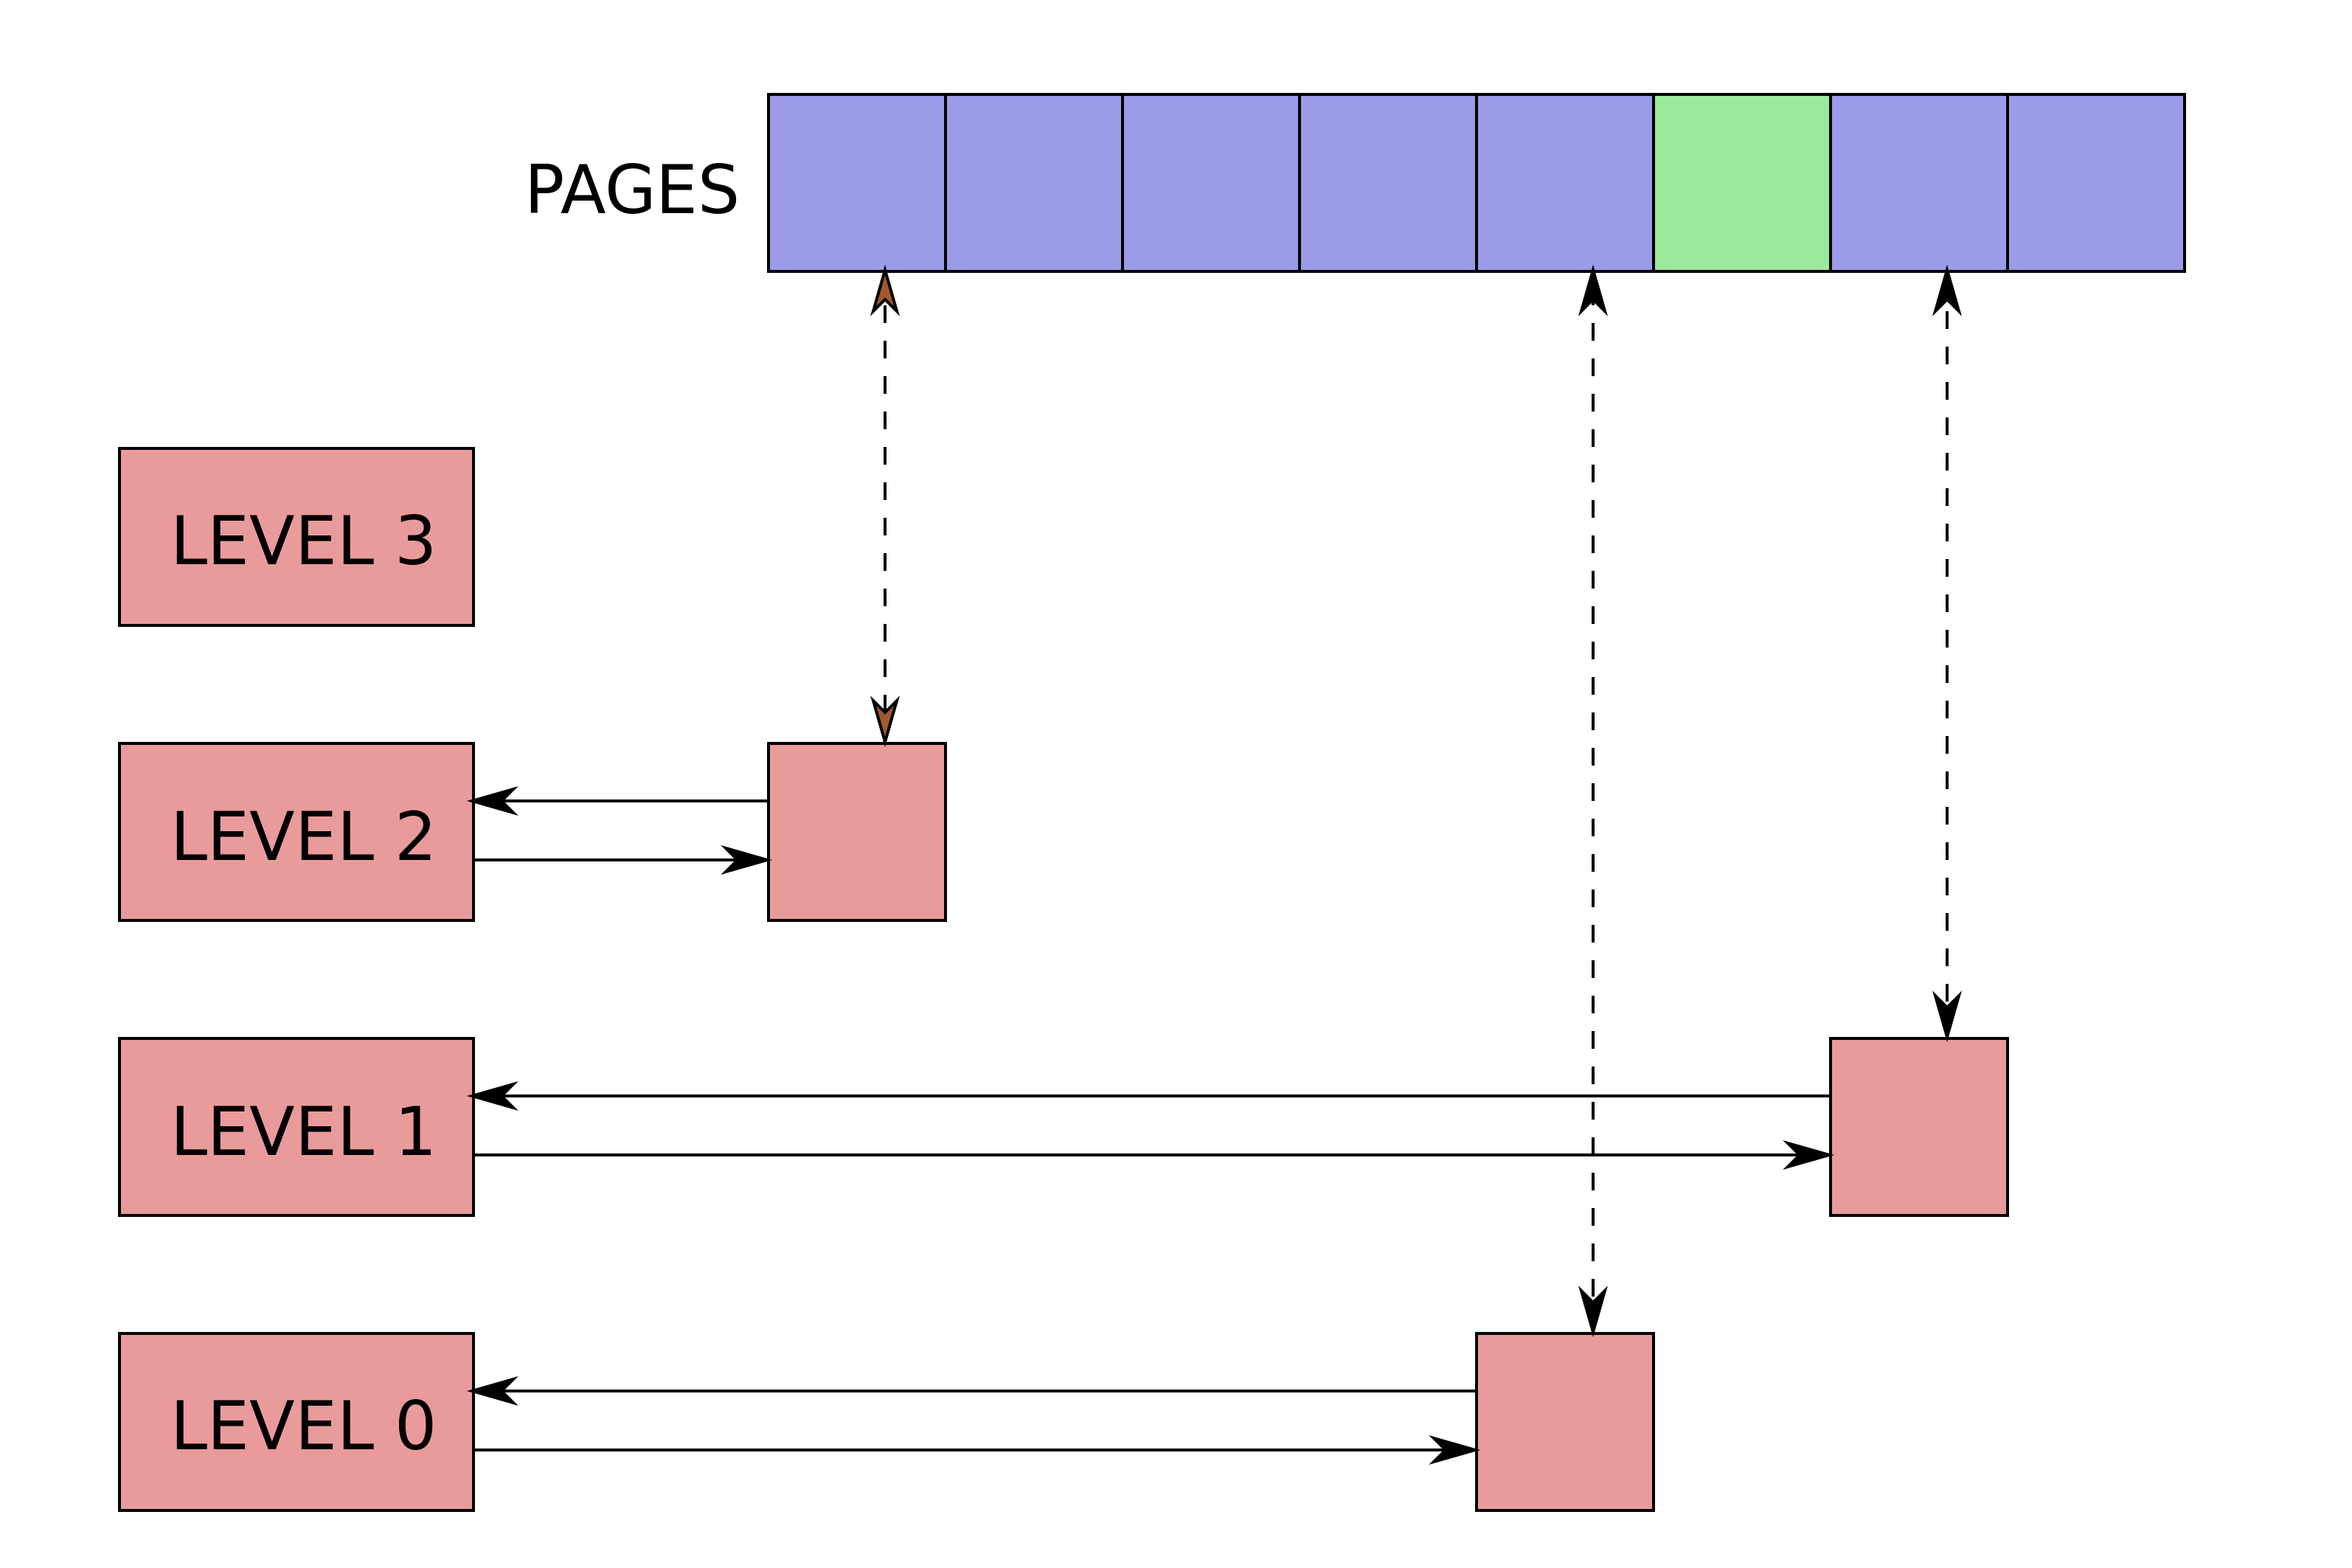
\includegraphics[height=.43\textheight]{bud5}
\end{frame}

  \begin{frame}
\frametitle{Кеширующий аллокатор}
\begin{itemize}
    \item<1->Создадим кеш блоков фиксированного размера
    \begin{itemize}
        \item<2->кеш будет аллоцировать/освобождать большие регионы памяти
        используя другой аллокатор;
        \item<3->кеш "нарезает" большие регионы на блоки фиксированного размера.
    \end{itemize}
\end{itemize}
\end{frame}

\begin{frame}
\frametitle{Кеширующий аллокатор}
\begin{itemize}
    \item<1->Кеширующий аллокатор имеет ряд достоинств:
    \begin{itemize}
        \item<2->фиксированный размер блоков позволяет бороться с фрагментацией;
        \item<3->аллокация/освобождение могут работать за $O\left(1\right)$;
        \item<4->можно скомбинировать кеши разных размеров и построить
        универсальный аллокатор.
    \end{itemize}
\end{itemize}
\end{frame}

\begin{frame}
\frametitle{SLAB}
\begin{itemize}
    \item<1->Кеширующий аллокатор предложенный Джеффом Бонвиком и
    использованный в SunOS (Solaris):
    \begin{itemize}
        \item<2->slab - описывает большой регион памяти, который разбивается на
        маленькие блоки фиксированного размера;
        \item<3->все свободные блоки связываются в список;
        \item<3->количество элементов списка и указатель на первый элемент
        сохраняются в заголовке.
    \end{itemize}
\end{itemize}
\end{frame}

\begin{frame}
\frametitle{SLAB}
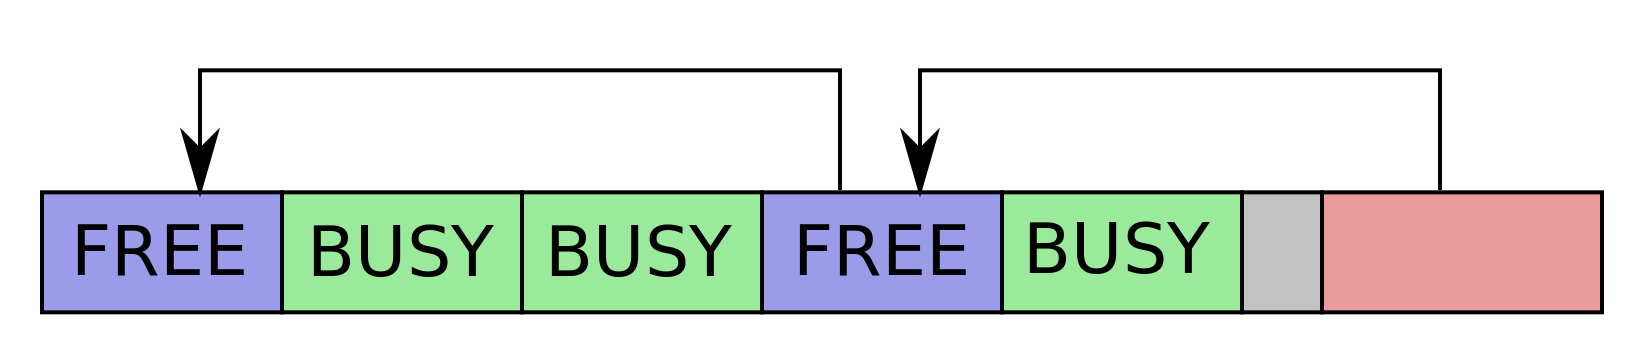
\includegraphics[height=.2\textheight]{slab0}
\end{frame}

\begin{frame}
\frametitle{Управление SLAB-ами}
\begin{itemize}
    \item<1->SLAB аллокатор управляет slab-ами:
    \begin{itemize}
        \item<2->если нет slab-а со свободными объектами - аллоцируем новый;
        \item<3->если все объекты в slab-е свободны - можно освободить slab.
    \end{itemize}
\end{itemize}
\end{frame}

\begin{frame}
\frametitle{Управление SLAB-ами}
\begin{itemize}
    \item<1->SLAB аллокатор поддерживает три списка slab-ов:
    \begin{itemize}
        \item<2->полностью свободные slab-ы;
        \item<3->частично знаятые slab-ы;
        \item<4->полностью занятые slab-ы.
    \end{itemize}
\end{itemize}
\end{frame}

\begin{frame}
\frametitle{Освобождение}
\begin{itemize}
    \item<1->Чтобы освободить элемент нужно найти slab, которому он пренадлежит
    \begin{itemize}
        \item<2->мы можем сохранить указатель на slab рядом с аллоцированной
        памятью;
        \item<3->мы можем потребовать чтобы размер и выравнивание slab-а были
        равны $2^i$.
    \end{itemize}
\end{itemize}
\end{frame}

\begin{frame}
\frametitle{Освобождение}
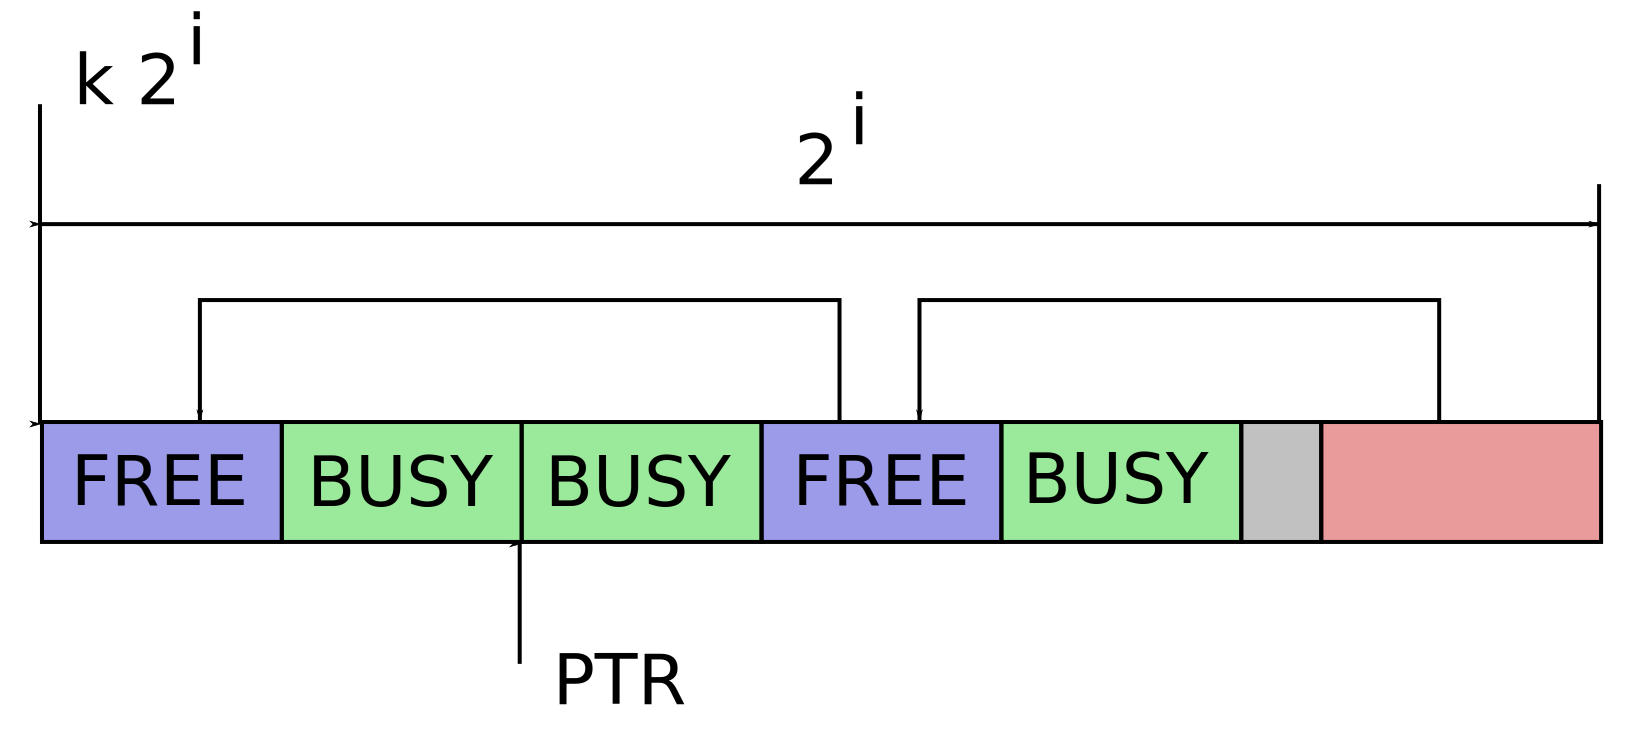
\includegraphics[height=.3\textheight]{slab1}
\end{frame}


\end{document}
